% This file is part of the stream_information project.
% Copyright 2017 the authors. All rights reserved.

% # style notes
% - it is Cram\'er--Rao not Cram\'er-Rao. And yet Fisher-matrix not Fisher--matrix.

\documentclass[modern]{aastex61}

% typography
\setlength{\parindent}{1.\baselineskip}
\newcommand{\acronym}[1]{{\small{#1}}}
\newcommand{\CRLB}{\acronym{CRLB}}
\newcommand{\FF}{\texttt{FAST FORWARD}}

% aastex parameters
%%\hypersetup{linkcolor=red,citecolor=green,filecolor=cyan,urlcolor=magenta}
\received{not yet; THIS IS A DRAFT}
%\revised{not yet}
%\accepted{not yet}
%% Adds "Submitted to " the arguement.
%\submitjournal{ApJ}
\shorttitle{information in stellar streams}
\shortauthors{bonaca et al.}

\usepackage{amsmath}

\begin{document}\sloppy\sloppypar\raggedbottom\frenchspacing % trust me

\title{The information content in cold stellar streams}

\correspondingauthor{Ana Bonaca}
% \email{whatevs}

\author[0000-0002-7846-9787]{Ana Bonaca}
\affil{Harvard--Smithsonian Center for Astrophysics}

\author[0000-0003-2866-9403]{David W. Hogg}
\affiliation{Center for Cosmology and Particle Physics,
Department of Physics,
New York University}
\affiliation{Center for Data Science,
New York University}
\affiliation{Flatiron Institute, Simons Foundation}
\affiliation{Max-Planck-Institut f\"ur Astronomie, Heidelberg}

\begin{abstract}\noindent % trust me
Cold stellar streams---produced by tidal disruptions of globular
clusters (or equivalent)---are long-lived, coherent dynamical features
in the stellar halo of the Milky Way.
They have delivered precise information about the mass distribution or
gravitational potential, including constraints on the shape of the
dark-matter halo.
Because of their different positions in phase space, different ages,
and different levels of observational scrutiny, different streams tell
us different things about the Galaxy.
Here we employ a Cram\'er--Rao (\CRLB) or Fisher-matrix approach to
understand the quantitative information content in the known
streams (Pal5, GD-1, Styx, [full list here]).
This approach depends on the existence of a generative model of
stellar streams, which we have developed previously, and which permits
easy calculation of derivatives of predicted stream properties with
respect to Galaxy model parameters.
We find that, in simple, static, analytic models of the Milky Way,
streams XX and YY contain the most information about the dark-matter
shape.
For any individual stream, there are near-degeneracies between
dark-matter halo properties and other parameters, including the mass
of the Large Magellanic Cloud, the total dark-matter mass, and other
potential parameters, but we find that simultaneous fitting of multiple
streams ought to precisely constrain all parameters well.
The \CRLB\ on any one parameter depends strongly on the model freedom;
as we permit more potential freedom, the information about, say, halo
triaxiality, reduces.
We perform experiments to demonstrate this using potential basis
functions that permit great freedom in the gravitational potential on intermediate
scales.
The \CRLB\ formalism also permits us to assess the value of future
measurements of stellar velocities, distances, and proper motions. We
make some comments about the information value of various new
observations that could be made of particular known streams.
\end{abstract}

\keywords{foo --- bar --- hello --- world}

\section{Introduction} \label{sec:intro}

\begin{itemize}
 \item establish streams useful in constraining gravitational potential
 \item tied to parametric models (too complex for inference otherwise, at least in current approaches)
 \item constraints only as good as the model (VL2 results)
 \item so, since not likely that the true potential is NFW, what are the streams actually constraining? 
 \item explicitly state this is the last use of toy models, used here to develop a framework, but should move to more flexible models in the future (DWH)
 \item here we're building a framework to measure the information content of stellar streams regarding the gravitational potential
 \item two-fold goals: given a simple parametric model, what kind of data do we need? what aspect of a (non-parametric) potential do individual streams constrain?
\end{itemize}


\section{Methods}
\label{sec:method}

\subsection{Information content in stellar streams}
Numerous methods have been developed to estimate properties of a dark matter halo by modeling observations of stellar streams \citep[e.g.,][]{}.
In this approach, the dark matter halo is usually described by an analytic model with a handful of free parameters.
We define the information content in this context as the best-case uncertainties on our model parameters achievable using the observational data at hand.
Formally, the lower bound on the variance of a deterministic parameter is given by the Cram\' er--Rao lower bound \citep[\CRLB,][]{Cramer1946, Rao1945}.

For some data set $\vec{y}$ (e.g., a vector of position and velocity measurements of stars along a stream), the associated covariance matrix is $C_y$.
Given the model parameters $\vec{x}$ (e.g., a vector with the mass and scale radius of a dark matter halo), the Cram\' er--Rao bound is the covariance matrix $C_x$.
The \CRLB\ is set by the inverse of a Fisher information matrix \citep{}:
\begin{equation}
C_x^{-1} = \left(\frac{d\vec{y}}{d\vec{x}}\right)^{T} C_y^{-1} \left(\frac{d\vec{y}}{d\vec{x}}\right) + V_x^{-1}
\label{eq:crlb}
\end{equation}
where $V_x$ is a covariance matrix containing the prior knowledge of model parameters.
In the next two subsections, we describe individual terms of Equation~\ref{eq:crlb}: model and its existing constraints (\S\ref{sec:model}), the change in stream observables $\vec{y}$ as a function of changes in the gravitational potential $\vec{x}$, i.e., the derivative $d\vec{y}/d\vec{x}$ (\S\ref{sec:derivatives}), and the adopted observational uncertainties, which set the covariance matrix $C_y$ (\S\ref{sec:datasets}).

\subsection{Model definition}
\label{sec:model}
The \CRLB\ formalism can only quantify information in the context of a model, which in our case is a model of a stellar stream in the gravitational potential of the Milky Way.
We consider cold stellar streams originating from disrupting globular clusters, which have been well-modeled with direct N-body simulations (refs).
These studies have shown that the phase-space distribution of the resulting debris is predominantly set by properties of the gravitational potential and the orbit of the progenitor, with a weaker dependence on the internal properties of the progenitor.
Hence, our model consists of parameters defining the gravitational potential and a 6-dimensional position of the progenitor.

To represent the global properties of the Milky Way, we represent the gravitational potential as a combination of a Hernquist bulge (parameterized with mass and scale radius), a Miyamoto-Nagai disk (with parameters for disk mass, scale length and scale height) and a spherical NFW halo (parameterized with scale velocity, scale radius, and axis ratios $q_x=q_z=1$).
We provide the fiducial values for this model in Table~\ref{t:model}, along with measurement uncertainties where available.
This potential is similar to MWPotential2014 \citep{galpy}, and fits a range observed Milky Way properties (e.g., rotation curve, ..., cit).

Next, we search for globular cluster orbits in the fiducial gravitational potential that produce stellar streams similar to those observed in the Milky Way.
Briefly, we use the streakline method to forward-model stream observations in a modification of the \FF\ framework from \citet{bonaca2014}.
For each stream, we vary the properties of its progenitor, while keeping the potential fixed at fiducial values.
Observations of all streams consist of on-sky positions of likely members, and their distance estimates from the location in the color-magnitude diagram.
Some streams have been better characterized, for example, with radial velocities from follow-up spectroscopy, and we include these extra dimensions of data in the parameter search if they are available.
In Appendix~\ref{sec:streams}, we provide current progenitor positions, initial masses and stream ages, which reproduce observations for most of the Galactic streams present in the PanSTARRS1 footprint, as well as more details on the above procedure.
When calculating the \CRLB\ for streams, we keep the progenitor mass and age fixed at their best-fitting values, as they are highly degenerate, and only use the present-day position of the progenitor as model parameters (defined in the observable space with the progenitor's two on-sky position angles, distance, radial velocity and two proper motion components). 

The complete model for measuring the information content in stellar streams has 15 parameters: nine for the distribution of matter in the Galaxy and six for the position of the stream progenitor (as defined in Table~\ref{t:model}).
Some of these parameters have already been measured, and we include these prior constraints as appropriate. 
For example, progenitors of streams are generally unknown, but several have been identified, such as globular clusters Palomar~5 and NGC~5466, and we include observational uncertainties on their position in our analysis through covariance matrix $V$ in Equation~\ref{eq:crlb}.
A substantial body of work has also been dedicated to constraining the mass components of the Milky Way.
As a result, properties of the bulge and the disk are known with a precision of x\% (cit) (from different kinds of study too?), which we include in covariance matrix $V$.
The halo mass, however, is still uncertain up to a factor of a few (cits), and the reported constraints on the halo shape are conflicting (cit), so the information that streams provide on the dark matter halo we measure independently of prior work.

\begin{center}
\begin{table}
\begin{tabular}{l c c c l}
\hline
\hline
Parameter & Symbol & Fiducial value & Uncertainty & Reference \\
\hline
\hline
Bulge mass & $M_b$ & & & \\
Bulge scale radius & $a_b$ & & & \\
Disk mass & $M_d$ & & & \\
Disk scale radius & $a_d$ & & & \\
Disk scale height & $b_d$ & & & \\
\hline
Halo scale velocity & $V_h$ & & & \\
Halo scale radius & $R_h$ & & & \\
Halo $y$ axis ratio & $q_y$ & & & \\
Halo $z$ axis ratio & $q_z$ & & & \\
\hline
Progenitor RA & $RA_p$ & & & \\
Progenitor Dec & $Dec_p$ & & & \\
Progenitor distance & $d_p$ & & & \\
Progenitor radial velocity & $V_{r,p}$ & & & \\
Progenitor RA proper motion & $\mu_{\alpha,p}$ & & & \\
Progenitor Dec proper motion & $\mu_{\delta,p}$ & & & \\
\hline
\hline
\end{tabular}
\caption{Model parameters}
\label{t:model}
\end{table}
\end{center}

\subsection{Calculating numerical derivatives for the \CRLB}
\label{sec:derivatives}
Intuitively, we can think of the Cram\'er--Rao bounds as quantifying how much we can change the parameters of a model $\vec{x}$, without violating the observational uncertainties of our data $\vec{y}$.
So, to calculate these bounds, we need the inverse of how much the observed quantities $\vec{y}$ vary as a function of model parameters $\vec{x}$, or formally the derivative $d\vec{y}/d\vec{x}$.
Given that in our case the data are a collection of points in a 6-dimensional space (3D positions and 3D velocities of stream members), this derivative becomes a non-trivial calculation.
In what follows, we describe how we measure differences in stream models with different input parameters.

\begin{figure}
\begin{center}
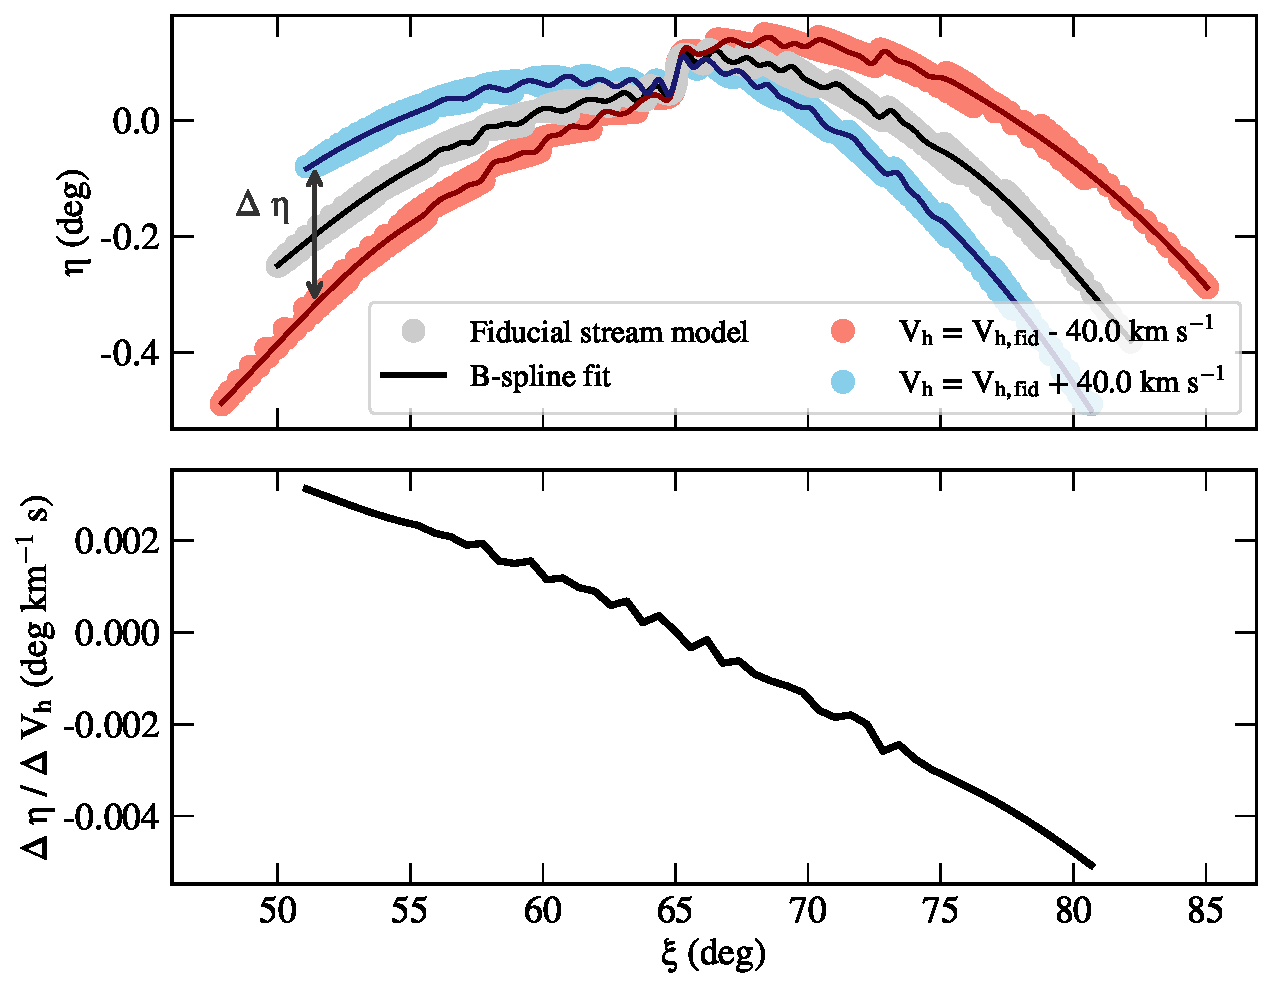
\includegraphics[width=0.8\textwidth]{derivative_vis.pdf}
\caption{We quantify the response of streams on changes in model parameters by calculating numerical derivatives, and in this figure we visualize the $d\eta / d V_h$ derivative (change in the sky position with the change in scale velocity of the underlying dark matter halo).
(\emph{Top}) The on-sky positions of the fiducial stream are shown in gray points, while the colored points show models in a less massive (red) and more massive halo (blue).
Solid lines show B-spline fits through these stream models.
The coordinate system is rotated such that the $\xi$ coordinate is approximately along the fiducial stream model, and $\eta$ is perpendicular to this stream track. 
(\emph{Bottom}) We define the derivative $d\eta / d V_h$ as the numerical derivative $\Delta\eta / \Delta V_h$.
At a fixed coordinate $\xi$ along the stream, the numerical derivative is the ration of the difference between $\eta$ coordinates of models in the more massive and the less massive halo ($\Delta\eta$, marked with arrows in the top panel), and the total difference in halo scale velocity between these two models ($\Delta V_h$).
This numerical derivative as a function of position along the stream is shown in a black line on the bottom panel.
}
\label{fig:derivative_steps}
\end{center}
\end{figure}

Cold streams analyzed in this work are very thin, most of them being at least two orders of magnitude longer than they are wide, and we treat them as one dimensional in the plane of the sky.
With each stream, we work in a spherical coordinate system ($\xi$, $\eta$) whose equator ($\eta=0$) is a great circle best-fitting the stream track, and the $\xi$ coordinate is our independent variable.
A detailed description of the great-circle fitting and a complete listing of rotation matrices for all of the analyzed streams are deferred until Appendix~\ref{sec:streams}, while an example of a resulting transformation is shown in Figure~\ref{fig:derivative_steps}, which shows positions of mock stream members in a rotated coordinate system.

We then measure deviations from the fiducial model at fixed positions along the stream ($\xi$), and use these numerical derivatives in our \CRLB\ calculation.
We illustrate the calculation of the $d\eta/d V_h$ derivative in Figure~\ref{fig:derivative_steps}, where in the top we show the on-sky position of a fiducial model in gray, and in red and blue models with a lower and higher halo scale velocity, respectively.
The numerical derivative at a position $\xi$ is then simply the difference between the $\eta(\xi)$ positions in the models of different scale velocity, divided by the difference in scale velocity between the models.
The bottom panel of Figure~\ref{fig:derivative_steps} shows how this derivative varies along the stream.
Derivatives in other data dimensions (distance, radial velocity, proper motions), and with respect to other model parameters, are calculated in the same fashion.
More formally, we calculate numerical derivatives using the following expression:
\begin{equation}
\left.\frac{d y_i}{d x_j}\right\rvert_{\xi_k} = \left.\left(\frac{y_i(x_{0,j} + \Delta x_j) - y_i(x_{0,j} - \Delta x_j)}{2\Delta x_j}\right)\right\rvert_{\xi_k}
\label{eq:derivative}
\end{equation}
where $y_i$ is the observable (either position $\eta$, distance, or one of the velocity components), $x_{0,j}$ is the fiducial value of parameter $x_j$, $\Delta x_j$ is a small value, and $\xi_k$ is the position along the stream where the derivative is evaluated.
A point to note is that we are not sensitive to changes along the stream within this formalism, which effectively reduces the dimensionality of our data, and might appear as not using the data to its full extent.
However, the coordinate along the stream (i.e., the stream length) is extremely correlated with the stream age, which is very poorly constrained with just the phase space distribution of the debris.
Consequently, not considering variations along the stream results in only a negligible loss of information.

\begin{figure}
\begin{center}
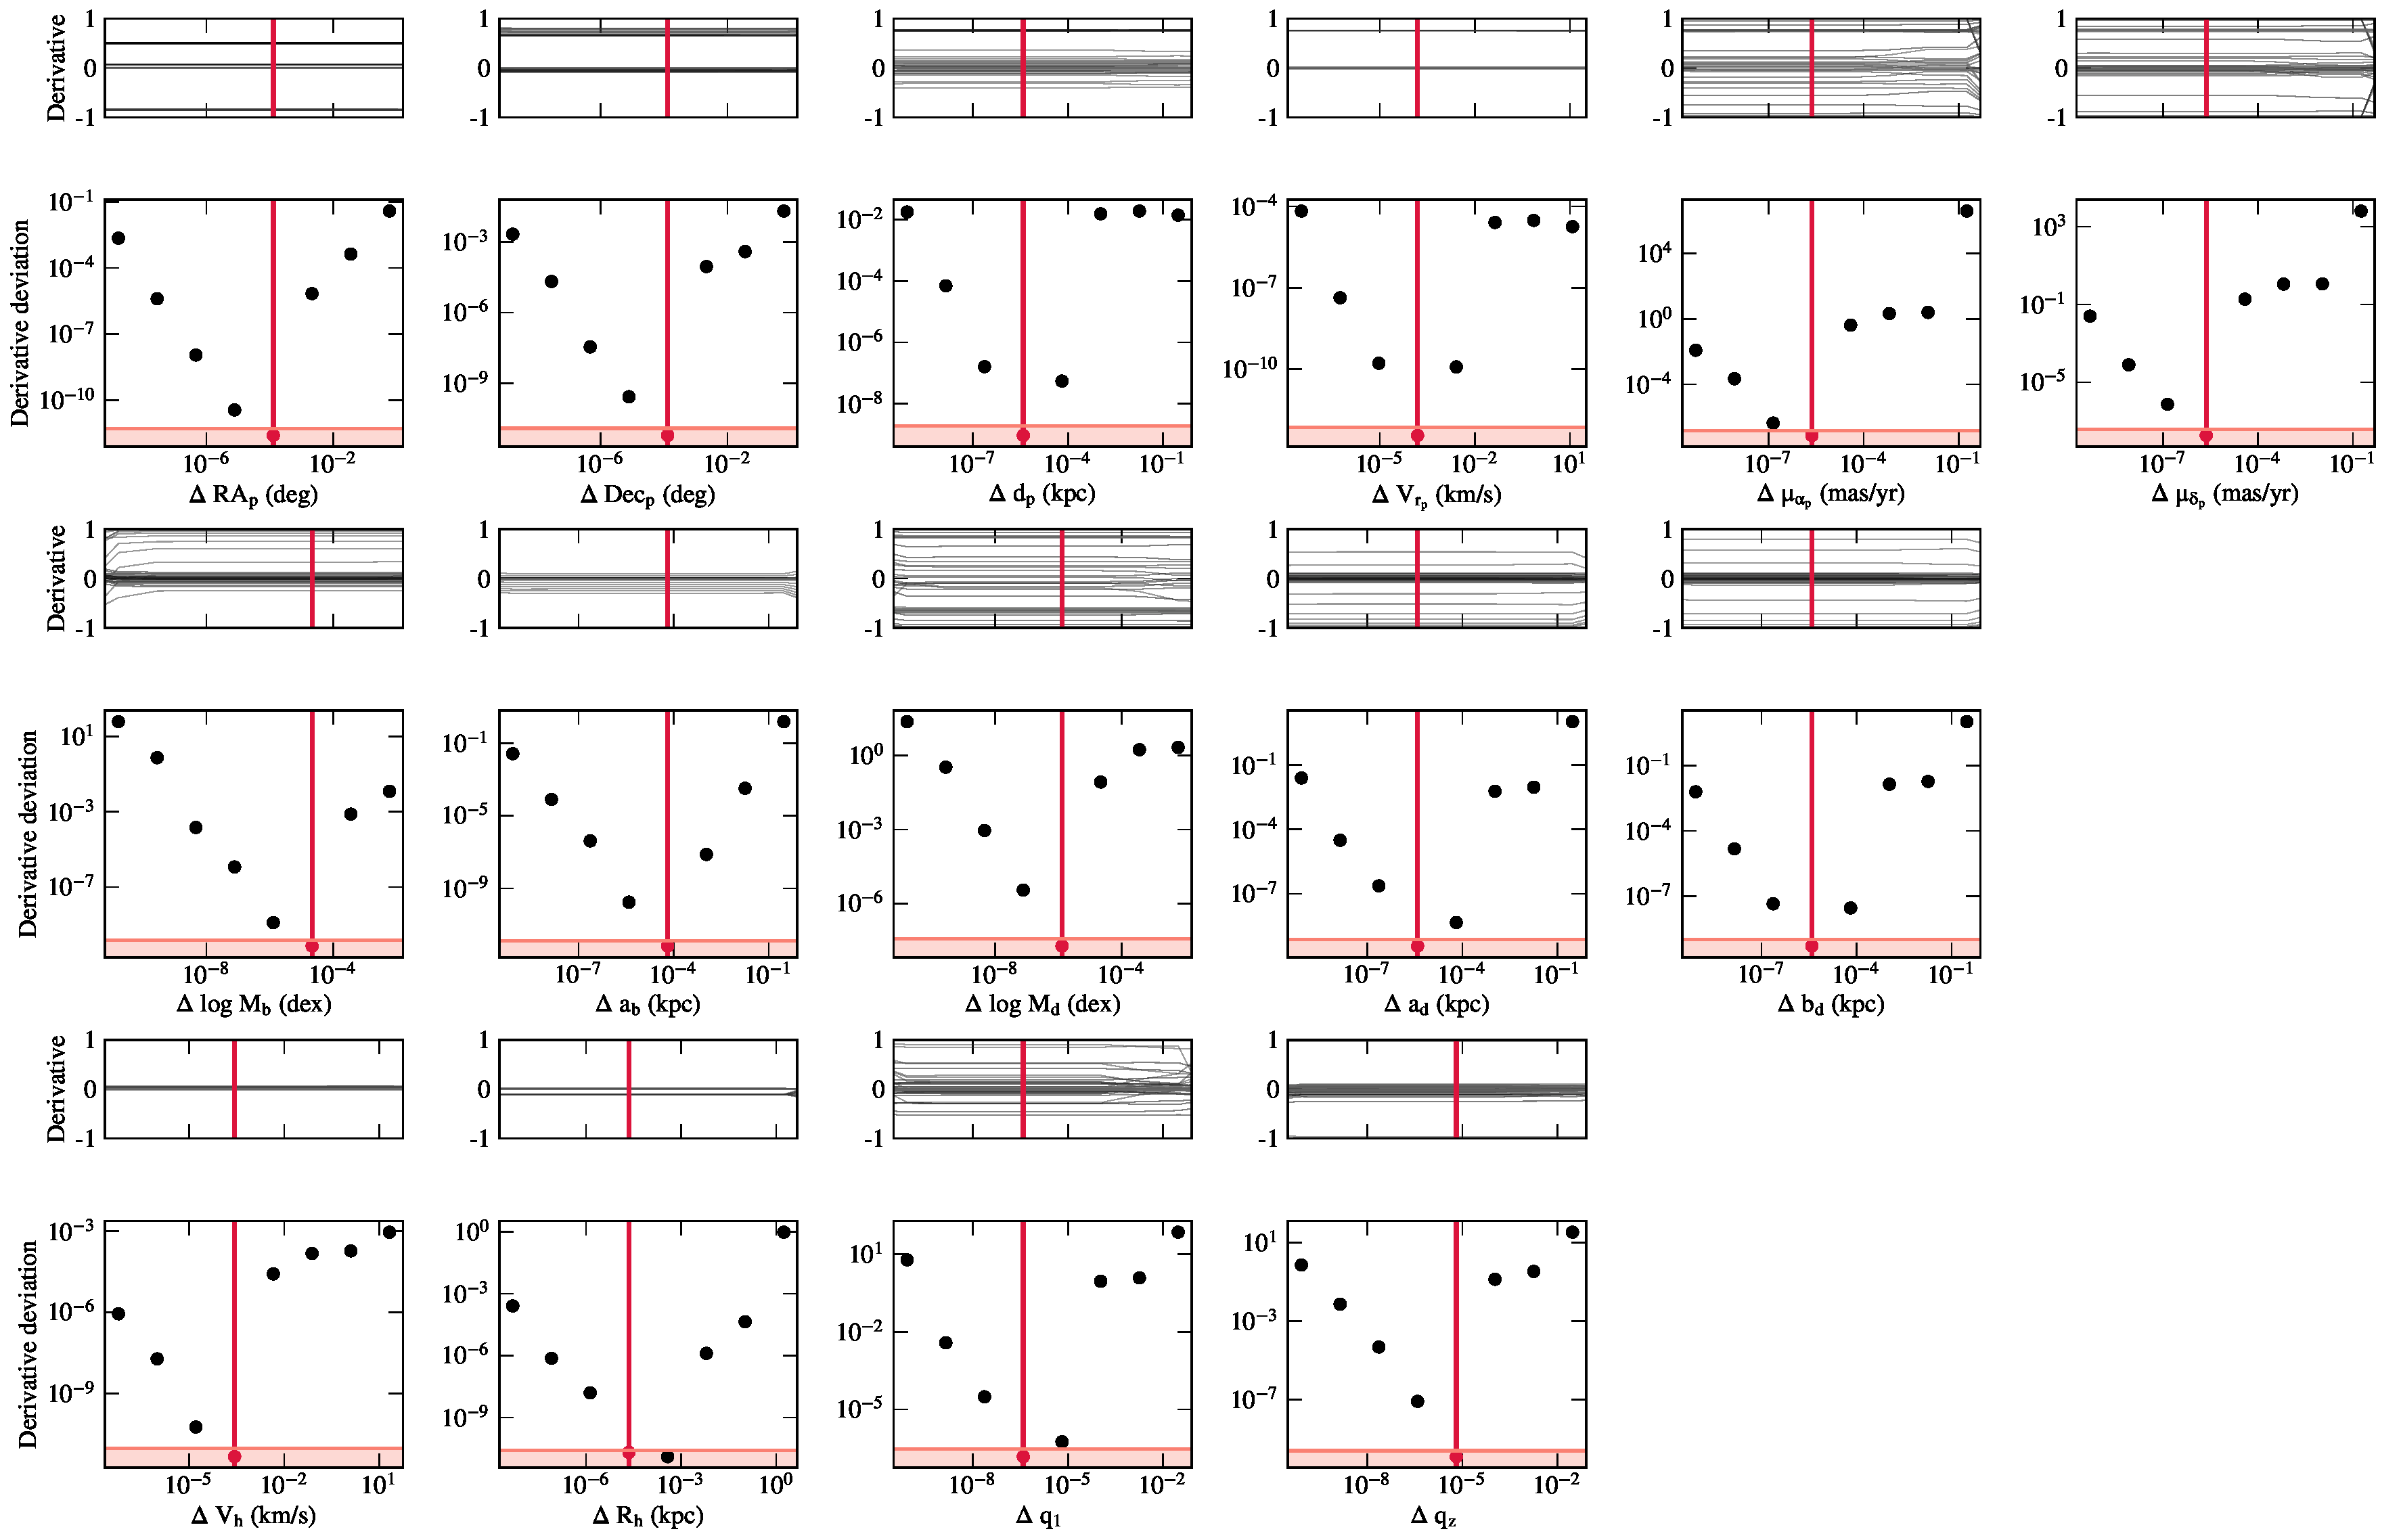
\includegraphics[width=\textwidth]{derivative_steps.pdf}
\caption{Optimal steps in parameter space for calculating numerical derivatives are marked with red vertical lines.
The top two rows present progenitor parameters, starting with progenitor position, $\rm RA_p$, on the left, until progenitor proper motion $\mu_p$ on the right.
The first of these two rows shows the values of evaluated numerical derivative, $\Delta y/\Delta x$, as a function of step size for parameter $x$ used in calculation, $\Delta x$, and the second row shows how the derivatives along the stream observables evaluated at a step size $\Delta x_j$ deviate from derivatives at adjacent step sizes $\Delta x_{j-1}$ and $\Delta x_{j+1}$.
Similarly, the middle two rows present derivatives for parameters defining the bulge and the disk, while the bottom two rows are dedicated to parameters of the dark matter halo.
For all of the model parameters, there is a local minimum in derivative deviation.
We adopt the optimal step size (red points and vertical lines) as the smallest step with a derivative deviation within a factor of 2 from the local minimum.
}
\label{fig:derivative_conv}
\end{center}
\end{figure}

The above prescription for calculating numerical derivatives relies (1) on the ability to evaluate any stream observable at a given position along the stream $\xi$, and (2) on the size of the parameter step $\Delta x$, and we now describe our strategies for addressing these points.
Both physical and model streams are a collection of stars, and thus all of the observables are discrete in nature (points in Figure~\ref{fig:derivative_steps}), which complicates comparison of different stream models.
However, to the first order, streams are one dimensional structures, and lines in the top panel of Figure~\ref{fig:derivative_steps} show that a B-spline fits well the distribution of stream positions.
We proceed by representing a stream model with a B-spline, which makes for a trivial evaluation of a stream observable at any position $\xi$.
This approach only takes into account information provided by the mean stream track, but not density variations along the track, and as such does not estimate the full information content in streams.
Nevertheless, the observed density variations along the streams are a convolution of true variations and observational incompleteness, which typically remains unconstrained.
Since the measurements of stream densities are uncertain, and we expect most of the information on the gravitational potential to be encoded in the stream track, in this work we focus on analyzing only the information content in the average positions of stream members, so approximating a stream model with a line is appropriate.

Finally, to robustly evaluate numerical derivatives entering the calculation of Cram\' er--Rao bounds, we explore how the derivatives depend on $\Delta x$, the parameter step size from Equation~\ref{eq:derivative}.
For every model parameter, we vary the step size by 10 orders of magnitude, store values of derivatives for different observables at several positions along the stream, and search for the step size where the derivatives are most stable.
Our metric for derivative stability at a step size $\Delta x_j$ is the overall deviation of derivatives evaluated at the adjacent step sizes $\Delta x_{j-1}$ and $\Delta x_{j+1}$, denoted $\Delta \dot{y}$ and defined as:
\begin{equation}
\Delta \dot{y} = \sum_i \left(\left.\frac{dy_i}{dx}\right\vert_{\Delta x_j} - \left.\frac{dy_i}{dx}\right\vert_{\Delta x_{j-1}}\right)^2 + \sum_i \left(\left.\frac{dy_i}{dx}\right\vert_{\Delta x_j} - \left.\frac{dy_i}{dx}\right\vert_{\Delta x_{j+1}}\right)^2
\label{eq:stability}
\end{equation}
where $y_i$ are observables (positions, distances and kinematics along the stream).
In Figure~\ref{fig:derivative_conv} we show numerical derivatives (short panels) and derivative deviations (square panels) as a function of parameter step size for the ATLAS-like stream in our sample.
Each row is dedicated to a group of parameters, with progenitor position on the top, parameters of the baryonic components in the middle, and parameters describing the dark matter halo in the bottom row.
At extremely large or small steps, the derivatives are unstable, which is evident as the derivatives themselves change (short panels), and also from their large deviations (square panels).
For all parameters, however, at intermediate step sizes the derivatives are constant and their deviations are small.
We adopt the smallest step size with a deviation within a factor of 2 from the minimum value (red point and vertical line) for calculating numerical derivatives.
Large deviations for large step sizes are due to derivatives being in the non-linear regime, while large deviations at small steps are reflecting the numerical noise.
The adopted step size is in between these two regimes, and is calculated for each stream individually.
For most parameters, the adopted size is rather small (e.g., on the order of $\rm m\,s^{-1}$ for velocities), but it still produces physically different stream models, underlying the importance of quantitative selection of step size in numerical differentiation.

While we presented a robust method to calculate numerical derivatives, a better solution would be to obtain derivatives directly when creating a stream model.
This is usually done using auto-differentiation, which has not been implemented in our legacy orbit integrator.
Evaluating exact derivatives of stream models with respect to input model parameters remains the most important technical improvement left for future work.


\subsection{Sets of observational data}
\label{sec:datasets}

\begin{table}
\begin{center}
\begin{tabular}{l c c c c c c}
\hline
\hline
Data set & $\sigma_\eta$ (deg) & $\sigma_d$ (kpc) & $\sigma_{V_r}$ (km\,s$^{-1}$) & $\sigma_{\mu_\alpha\star}$ (mas\,yr$^{-1}$) & $\sigma_{\mu_\delta}$ (mas\,yr$^{-1}$) \\
\hline
Fiducial & 0.1 & 2.0 & 5 & 0.1 & 0.1 \\
DESI & 0.1 & 2.0 & 10 & N/A & N/A \\
Gaia & 0.1 & 0.2 & 10 & 0.2 & 0.2 \\
Extragalactic & 0.5 & N/A & 20 & N/A & N/A \\

\hline
\hline
\end{tabular}
\caption{Observational data sets}
\label{t:datasets}
\end{center}
\end{table}

The amount of information we can learn about the gravitational potential from a stream data set depends both on the intrinsic sensitivity of a stream on different aspects of the gravitational potential, and also on the properties of the data set itself.
The intrinsic sensitivity, encoded in the derivatives of stream observables with respect to potential parameters, has been discussed above.
In this section, we set up different stream data sets, defined by the type, amount and precision of observations at hand.

For simplicity, we assume that observations are uniformly distributed every 0.5\,deg along each stream, with a minimum of 15 measurement points per stream.
We also assume that all the different types of data (e.g., radial velocity, proper motions) are measured at these same positions along the stream and that the uncertainties are the same for a given type of observation.
All of these assumptions make for a highly idealized scenario: there are density inhomogeneities along the streams, so the likely members are hardly equidistant; different types of data are typically obtained for different stars; and observational uncertainties are a function of stellar brightness, color, and often distance.
However, in this work we merely aim to demonstrate a framework for calculating the information content of a stream data set.
More realistic data can be analyzed in the same way to produce tailored predictions.

In measuring the information content in the Milky Way streams, we consider the following scenarios of data availability:
\begin{enumerate}
\item fiducial data set obtainable with targeted kinematic follow-up,
\item present data on positions of stream stars with radial velocities from DESI and DESI-like surveys,
\item data on stream members from the final data release of the Gaia mission, and
% \item integrated-light data, as available for extragalactic streams.
\end{enumerate}
Observational uncertainties in each of these cases are summarized in Table~\ref{t:datasets}, and described in more detail below.

For the fiducial data set, we assume that the positions of stream members come from photometric surveys, radial velocities from targeted spectroscopic follow-up, and proper motions from long-baseline, spacecraft observations.
The on-sky positions of stars are measured very precisely (for example, better than 0.5\,'' in SDSS, cit), so the uncertainty in stream position equals the stream width.
Globular clusters produce thin streams, and the ones discovered so far vary between x deg (stream, ref) to y deg (stream, ref).
We adopt 0.1 deg for our fiducial positional uncertainty.
Unlike the positions projected on the sky, the distances to most of the streams are highly uncertain, as there are typically no standard candles identified along the stream.
The main distance indicator is merely the position of the main sequence turn-off, which, assuming the stellar population age and metallicity are known, provides a distance uncertainty of $\sim20\,\%$.
For simplicity, we adopt a single value of $2\,\rm kpc$ as our fiducial uncertainty in distance, which is conservative for nearby streams, but perhaps overly optimistic for the more distant ones.
On the kinematics side, our fiducial uncertainty for radial velocities is 5\,km\,s$^{-1}$, as a number of medium-resolution spectrographs have demonstrated such performance (cit).
And finally, space-based astrometry with a long baseline allows proper motions to be measured with an uncertainty of only 0.1\,mas\,yr$^{-1}$, which we also use as our fiducial uncertainty (cite Sohn Sgr paper).
These uncertainties, especially for the kinematics, are currently best attainable.
Most of the streams, however, only have positional data, and only a few have kinematic information from radial velocities.
So within the fiducial case, we consider separate situations of having access to 3D (positions only), 4D (positions and radial velocities) and 6D data (full phase space).

In the second case, we emulate a data set whose positions originate from photometric surveys, same as in the fiducial case, but which includes radial velocities from lower-resolution spectroscopic surveys.
We study this scenario in anticipation of a number of highly multiplexed, $R\approx5,000$ surveys being launched in the next few years (e.g., DESI, cit).
These surveys were designed to target objects as faint as $g=20$, and are expected to deliver radial velocities for the Milky Way sources with an uncertainty of 10\,km\,s$^{-1}$.
Albeit this value, which we adopt for this case, is an order of magnitude worse than the radial velocity precision in our fiducial case, these surveys will operate very quickly, and have the potential to provide kinematics for all of the known streams -- a feat hard to accomplish with targeted follow-up.
With this scenario, we will specifically explore whether it is more informative to have precise radial velocities for a few streams or less precise data for many streams.

Our final case studies data in the post-Gaia era, where distances come from Gaia parallaxes, radial velocities from Gaia's Radial Velocity Spectrometer (RVS), and proper motions from the 5-year Gaia astrometry.
The uncertainty in stream position will still be limited by its intrinsic width, but the distance estimates should be improved by an order of magnitude with respect to the fiducial case.
Typical Gaia parallax uncertainty for bright red giants is 0.01\,mas\,yr$^{-1}$ at the end of mission (cit), which translates to a distance uncertainty of 1\,kpc at 10\,kpc.
Distance precision is expected to increase by a factor of 5 after matching the astrophysical parameters of these stars (cit), so we use 0.2\,kpc as our distance uncertainty.
For a similar population of stars, RVS will deliver radial velocities precise to 10\,km\,s$^{-1}$.
Lastly, proper motion precision is $\approx0.2$\,mas\,yr$^{-1}$ for faint, blue stars, such as those at the main sequence turn-off of stellar streams.
We adopt this value for our proper motion uncertainty, as we expect faint blue stars to make up the majority of identified stream members.
Data in this scenario are assumed to span the full phase space, and are distinguished from the fiducial 6D case only by the expected measurement uncertainties.
Distances are slightly more precise, while the kinematics are a factor of 2 worse than in the fiducial case, so when comparing the two, we will be able to gauge relative importance of different types of data for dynamical modeling of streams.


\section{Results}
Following the steps outlined in section~\S\,\ref{sec:method}, we inferred the information content in 11 Milky Way-like streams.
In this section, we first present constraints on the underlying gravitational potential from a single stream (\S\,\ref{sec:res_ind}), then compare constraints from different streams (\S\,\ref{sec:res_comp}), and finally explore joint constraints from multiple streams (\S\,\ref{sec:res_joint}).

\subsection{Individual stream}
\label{sec:res_ind}

\begin{figure}
\begin{center}
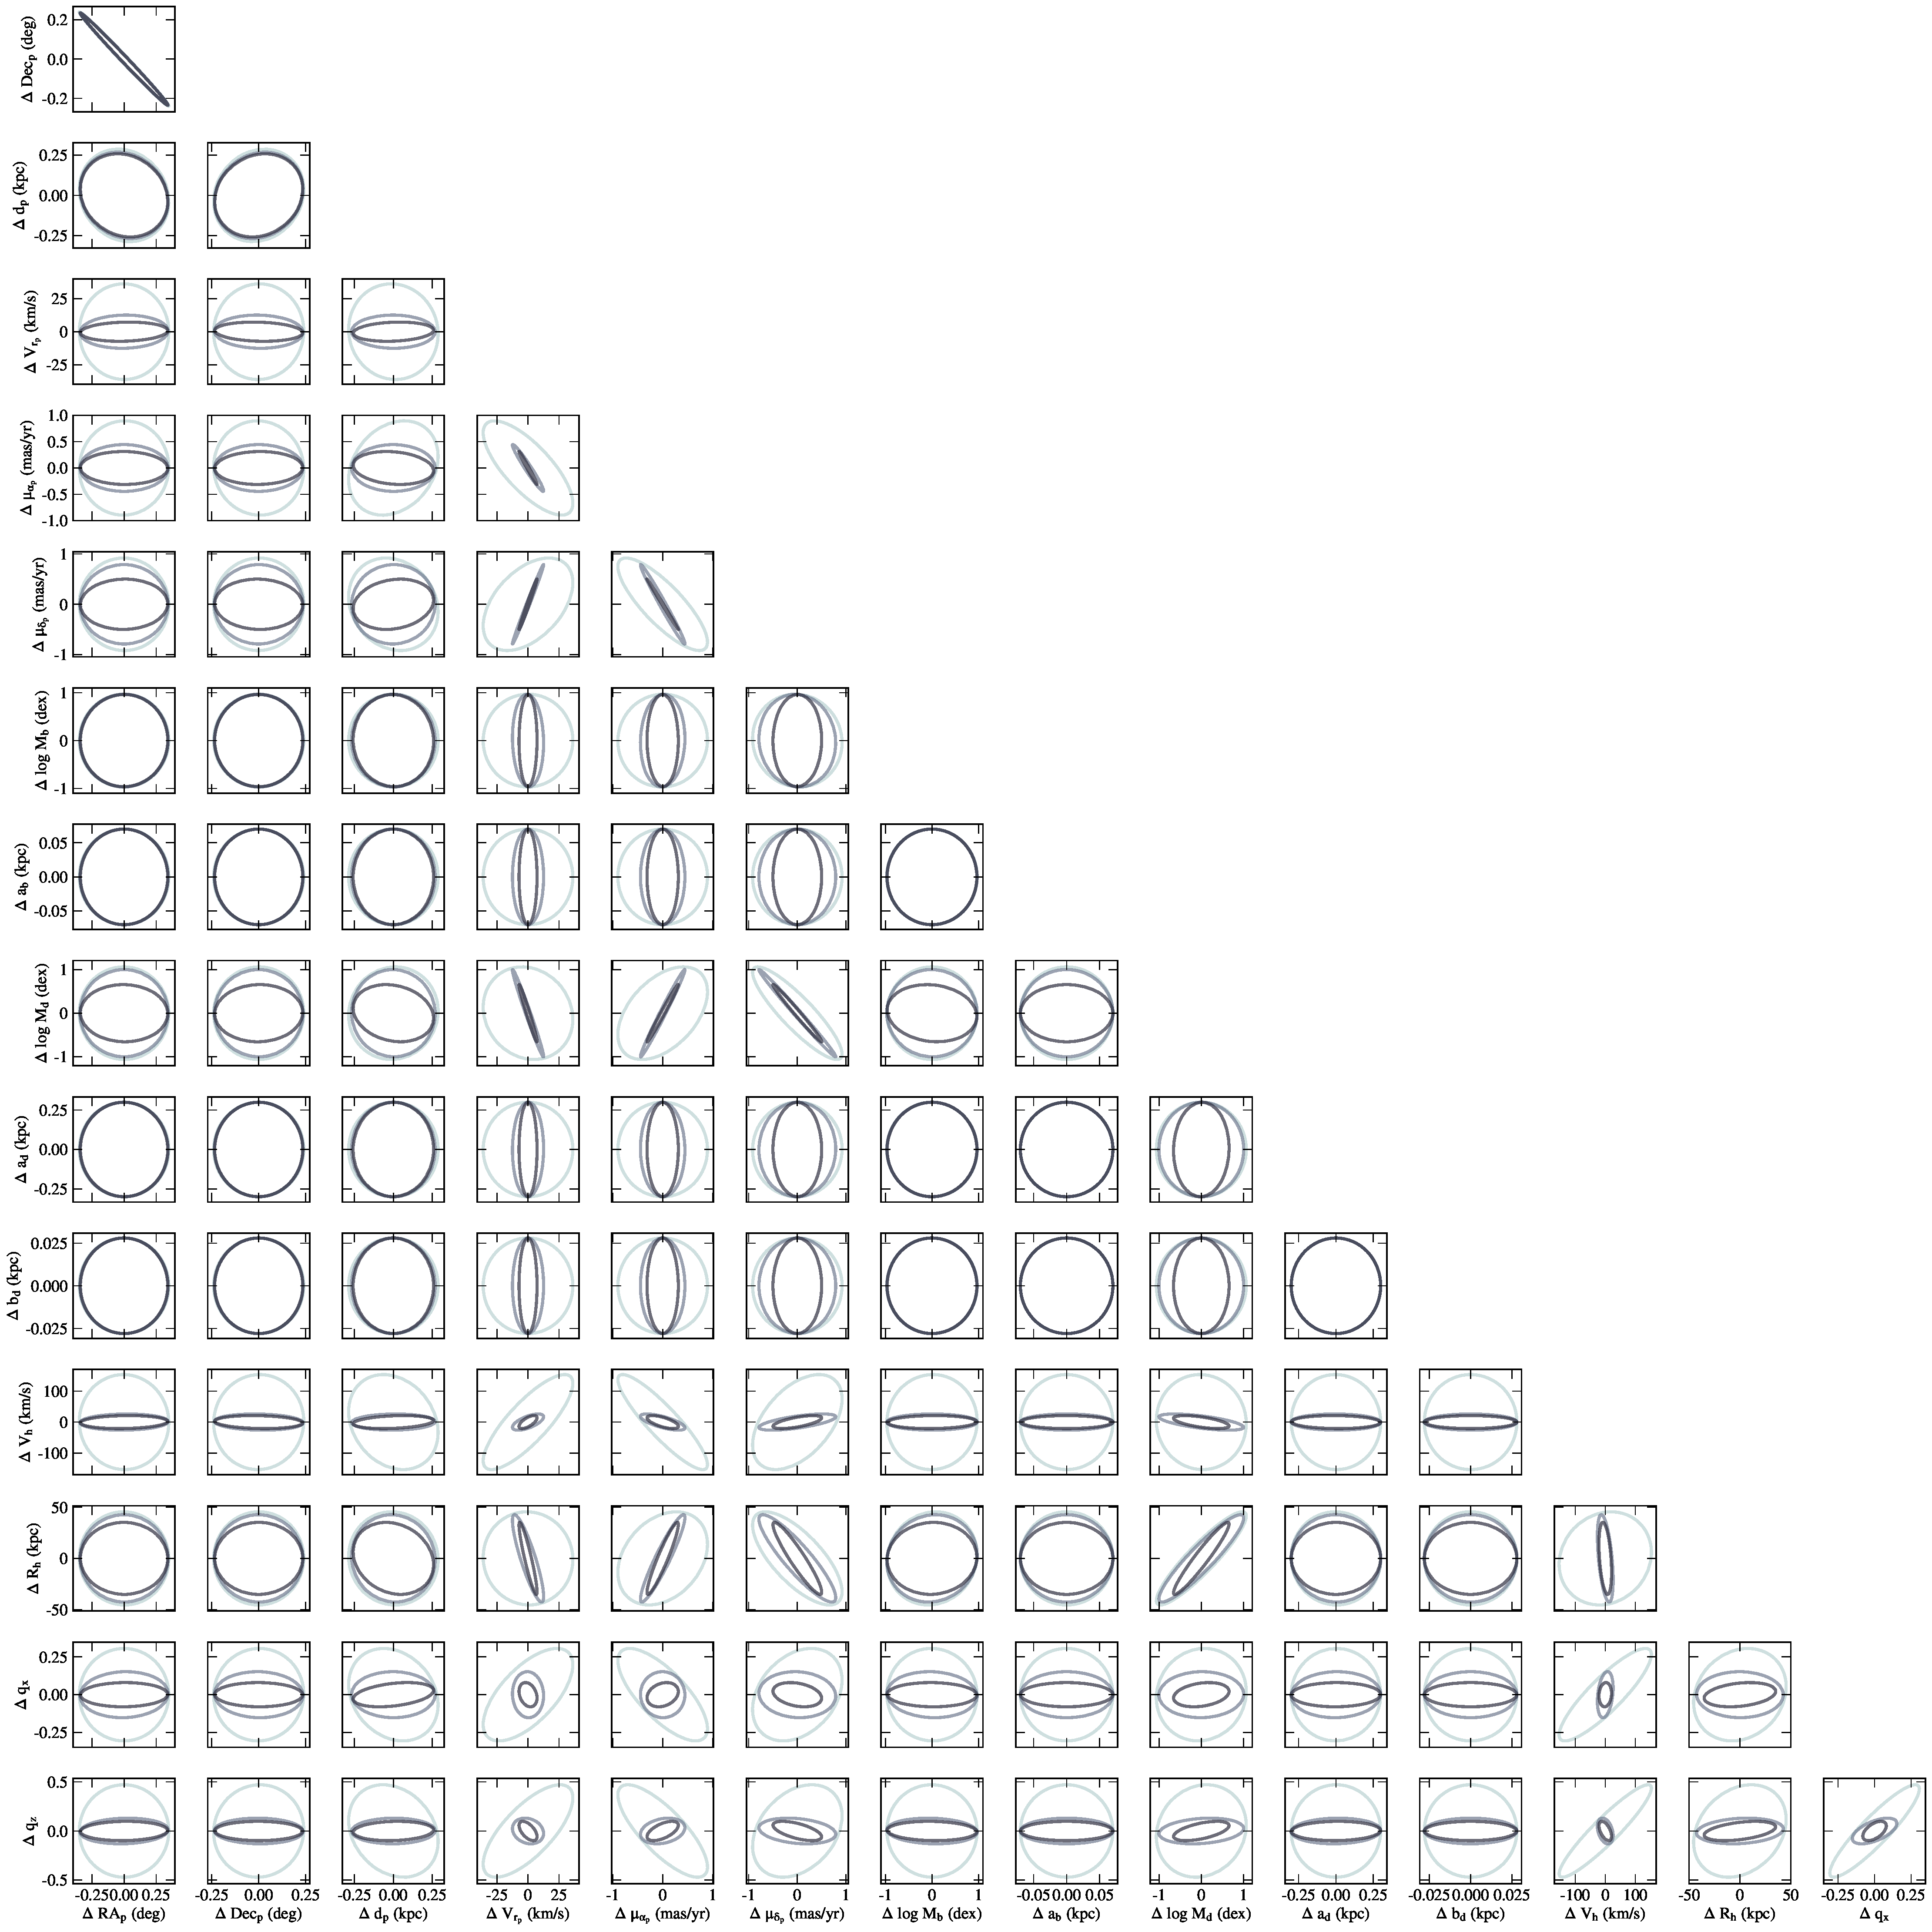
\includegraphics[width=\textwidth]{crb_correlations.pdf}
\caption{A visualization of correlations between Cram\'er--Rao bounds (ellipses) on all 15 of the model parameters for an ATLAS-like stream.
The lightest colored ellipses show constraints achievable when only on-sky positions and distances are known, medium shaded ellipses are constraints produced with an addition of radial velocities, while the darkest ellipses are constraints with the full 6-D phase space information on stream members.
The addition of kinematic data drastically improves constraints on most of the parameters, indicating that kinematics are essential for meaningful recovery of the Galactic potential.
However, streams seem to contain little information on the baryonic matter components of the Galaxy -- these constraints do not improve with more data and remain prior-dominated.
}
\label{fig:crb_correlations}
\end{center}
\end{figure}

We estimate how precisely every stream data set constrains the current position of the stream's progenitor, as well as the underlying gravitational potential.
For a given combination of a stream and an observational set up, all of this information is contained in a 15~by~15 Fisher matrix $C_x$.
In Section~\ref{sec:method}, we showed how to calculate the inverse of the Fisher matrix $C_x^{-1}$ (Equation~\ref{eq:crlb}).
If the condition number of $C_x^{-1}$ is small, it can be easily inverted to obtain the Fisher matrix.
However, when the model parameters are poorly constrained, $C_x^{-1}$ has a large condition number, and it is then non-invertible by standard libraries.
We find that condition numbers of calculated $C_x^{-1}$ tend to be large, so to get the Fisher matrix $C_x$, we use a robust, iterative method of matrix inversion, described in Appendix~\ref{sec:inversion}.

Once we have the Fisher matrix, the square root of its diagonal are the CRLB, which measure the best attainable precision in the 15 parameters of our model.
If all of the model parameters were uncorrelated, the Fisher matrix would be diagonal.
However, we find that Fisher matrices have off-diagonal elements for all of the streams, and in the remainder of this section, we discuss covariances between different model parameters inferred from observations of an ATLAS-like stream.

The corner plot in Figure~\ref{fig:crb_correlations} visualizes the structure of the Fisher matrix for an ATLAS-like stream, under the assumption of fiducial observational uncertainties.
Ellipses in each panel show covariant CRLB for a single pair of model parameters, with different colors indicating the dimension of the assumed fiducial data set: the lightest ellipses are constraints from 3D positions only, the medium ellipses include 3D positions and radial velocities, and the darkest ellipses are for the full 6D fiducial data set.
Properties of an ellipse for a pair of parameters $i,j$ are determined from a slice of the Fisher matrix $C_x$ such that its rotation angle $\theta$, width $w$ and height $h$ are given by:
\begin{align*}
\theta &= {\rm arc tan}\left(\frac{V_{1,0}}{V_{0,0}}\right) \\
w &= 2\,\sqrt{v_0} \\
h &= 2\,\sqrt{v_1}
\end{align*}
where $V_k$ are the eigenvectors ($V_{k,l}$ is the $l$ component of the eigenvector $k$) and $v_k$ the corresponding eigenvalues of the Fisher-matrix slice $M_{ij} \equiv \left[\left[C_{x,ii}, C_{x,ij}\right], \left[C_{x,ji}, C_{x,jj}\right]\right]$.

In general, additional stream data leads to tighter constraints on model parameters, and consequently darker ellipses in Figure~\ref{fig:crb_correlations} are smaller than lighter ellipses, although the relative sizes vary between different pairs of parameters.
In some cases, the impact of additional data is drastic.
For example, the presence of radial velocities in a data set collapses the uncertainty in the progenitor radial velocity, $V_{r_p}$, by an order of magnitude (compare the lightest and medium-colored ellipses in the fourth column from the left in Figure~\ref{fig:crb_correlations}).
For other parameters, additional data can break degeneracies existing in bounds from less extensive data sets, such as that between the halo scale velocity, $V_h$, and halo $x$-axis ratio, $q_x$, which are tightly correlated when constrained by a 3D data set, but show hardly any correlation when analyzed with 6D data (see panel in the second row from the bottom, and the third column from the right).
Typically however, additional data only tightens parameter constraints, and keeps the correlations between parameters in place.
Finally, for some parameters, additional data provides almost no additional constraints.
For the ATLAS-like stream presented in Figure~\ref{fig:crb_correlations}, additional data has no impact on the on-sky position of the progenitor, which is mainly inferred from the on-sky positions of stream stars, as well as on some bulge and disk properties, which are dominated by the prior.
Given that the pericenter of this stream is 23\,kpc, which is approximately 30 and 7 times beyond the bulge and disk scale lengths, respectively, it is unsurprising that its debris provides little information on these components.
This example serves a cautionary tale -- obtaining additional data along a stream can be expensive, so it is important to quantify the expected gains beforehand, and we have provided a framework to do so.

Data sets featuring only positions of stream stars, provide weak, but not vanishing, constraints on model parameters.
This result is somewhat surprising, because in the absence of kinematics, the masses and timescales in the system can be arbitrarily rescaled to reproduce the same positions, so we expect that kinematic data is a prerequisite for any dynamical inferences.
However, we introduced a mass scale in the problem by fixing the mass of the stream progenitor, rather than using it as a model parameter.
This effectively assumes infinitely precise knowledge of the progenitor mass, which likely propagates into weak constraints on model parameters, as obtained in the absence of kinematic data.
Since these constraints from 3D data are much weaker than those from 4D and 6D data sets, we decided not to complicate our analysis by an introduction of another parameter, and simply note that they are driven by the prior knowledge of the progenitor properties.
% To corroborate the relation between kinematics and precision in mass estimates, we note that adding radial velocities to positions alone decreases the uncertainty in estimated halo mass (predominantly set by the halo scale velocity $V_h$) by an order of magnitude.

As the final element of our exploration of a Fisher information matrix for a single stream, we discuss correlations between constraints on different parameters.
The CRLB ellipses in different panels of Figure~\ref{fig:crb_correlations} exhibit the whole range of correlations: from strongly and mildly (anti-)correlated, to those completely uncorrelated.
We quantify these covariances with the Pearson correlation coefficient, which for a pair of parameters $(i,j)$ is simply $p = C_{x,ij} / \sqrt{C_{x,ii}\,C_{x,jj}}$, where $C_{x,kl}$ is the $k,l$ element of the Fisher matrix $C_x$.
We report correlation coefficients for parameters constrained with 6D fiducial data set in the upper right corner of each panel in Figure~\ref{fig:crb_correlations}, and discuss below the most extreme values.

On-sky positions of an ATLAS-like progenitor are perfectly anti-correlated, which reflects this stream's one-dimensional nature and its projected span from southeast to northwest.
Similarly, the progenitor's proper motions are anti-correlated, indicating that at least one component of the velocity vector is aligned with the stream.
This is further supported by the strong correlations between progenitor's proper motions and its radial velocity -- a mark that there is a more physical decomposition of progenitor's velocity vector.
One would expect similar behavior for the 3D spatial position of the progenitor, however, distances in our fiducial case are too uncertain to exhibit correlations with on-sky positions.

In addition to correlations arising from the geometry of stream observations, there are also covariances originating from the physical aspects of stream constraints on the gravitational potential.
For example, scale velocity and scale radius of the dark matter halo are mildly anti-correlated, which is expected if the stream is most sensitive to the total amount of matter within the volume it orbits, but is somewhat agnostic to the distribution of matter.
In order to conserve the total mass in the halo, $M_h \propto V_h^2\,R_h$, the halo scale velocity needs to decrease as its scale radius increases, so the correlation between these two parameters is negative.
On the other hand, streams provide little additional information regarding the bulge and disk parameters, so most of them are constrained by the priors alone and decoupled from other parameters.
However, the disk mass is mildly anti-correlated with the halo scale velocity, and strongly correlated with the halo scale radius.
This can again be understood in the context of streams only constraining the mass enclosed within their orbits, because as the halo scale radius increases, or the halo scale velocity decreases, the mass of the inner halo decreases.
The total enclosed mass has a halo and a disk contribution, so if the halo component decreases, the disk must increase, which then introduces the observed correlations between the halo and disk parameters. 

There are also strong correlations between the halo scale radius and the progenitor's kinematics.
These underscore the importance of including the progenitor parameters in measuring the information content in stellar streams, as neglecting to do so would lead to overly optimistic estimates.
Furthermore, this mixing between parameters describing the progenitor and those describing the distribution of matter indicate that some streams might be at a more informative orbital phase or position relative to the Sun, a prospect we investigate in the next section where we compare stream performance in constraining parameters of the gravitational field.

\subsection{Comparison between streams}
\label{sec:res_comp}
In the context of our model, each stream provides information on the position of its individual progenitors, as well as on the distribution of matter in the Galaxy that they all measure in common.
In this section, we discuss how constraints on various aspects of the Galactic gravitational field compare between 11 streams in our sample.

\begin{figure}
\begin{center}
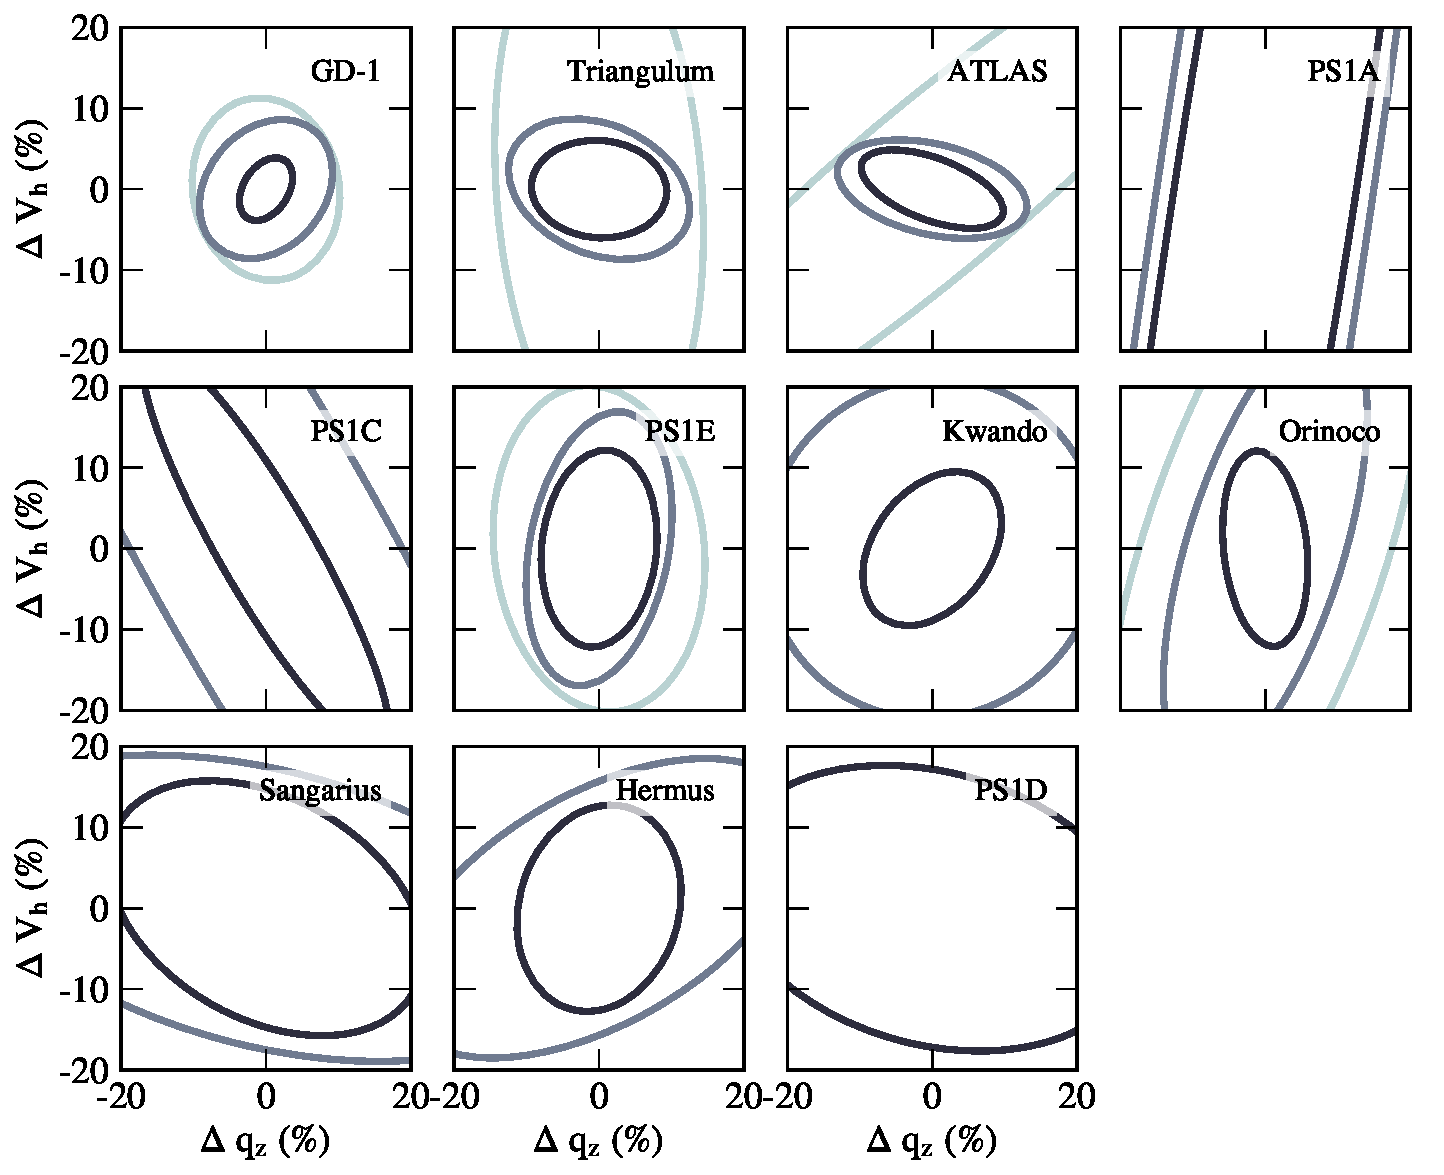
\includegraphics[width=\textwidth]{crb2d_allstream.pdf}
\caption{Fractional Cram\'er--Rao bounds on the scale velocity and $z$-to-$y$ axis ratio of the dark matter halo, based on fiducial observations of 11 streams in our sample.
The lightest ellipses represent constraints from 3D spatial data, medium ellipses include information from radial velocities in addition to positions, and the darkest ellipses feature data sets with full 6D phase-space.
The quality of constraints varies among the streams from GD-1, where the constraints are within 20\% in every case considered, to PS1-D, for which only the 6D data set provides constraints better than 20\%.
The two halo parameters are differently correlated, so combining multiple streams will break some of these individual degeneracies.
}
\label{fig:crb2d_comparison}
\end{center}
\end{figure}

In previous section, we explored correlations in Cram\' er--Rao bounds between all parameter pairs (Figure~\ref{fig:crb_correlations}), so we start this section by comparing different streams' constraints on a pair of parameters.
Figure~\ref{fig:crb2d_comparison} features 2D Cram\' er--Rao bounds for the halo scale velocity and its $z$-axis flattening, with each panel in a grid dedicated to a single stream.
Analogously to Figure~\ref{fig:crb_correlations}, light, medium through dark ellipses are constraints based on 3D, 4D and 6D fiducial data sets, respectively.
Unlike the previous figure, here the parameter constraints are relative, and capped at 20\,\% to highlight the most informative streams.
Performance of different streams in constraining halo scale velocity and halo shape varies from better than 20\,\% with only 3D data for streams such as GD-1 and PS1E, to worse than 20\,\% for PS1D even with 6D data, and everything in between.
Relative importance of the input data also varies among the streams; for example, additional radial velocities improve constraints from GD-1 only marginally, but they provide a major improvement in constraints from Triangulum and ATLAS.
An in-depth analysis of these bounds can inform an optimal observing strategy, and we explore implications that currently ongoing spectroscopic and astrometric surveys will have for tidal streams in Section~\S\,\ref{sec:forecast}.
Constraints on halo scale velocity and shape are correlated for all of the streams, but these correlations differ in both degree and direction.
In the following section, we investigate how combining different streams can break these degeneracies.
In the remainder of this section, we examine why different streams are differently sensitive to various model parameters, and study how \CRLB\ for individual parameters depend on properties of the stream and the orbit of its progenitor.

\begin{figure}
\begin{center}
\includegraphics[width=\textwidth]{crb_onsky_gal1.pdf}
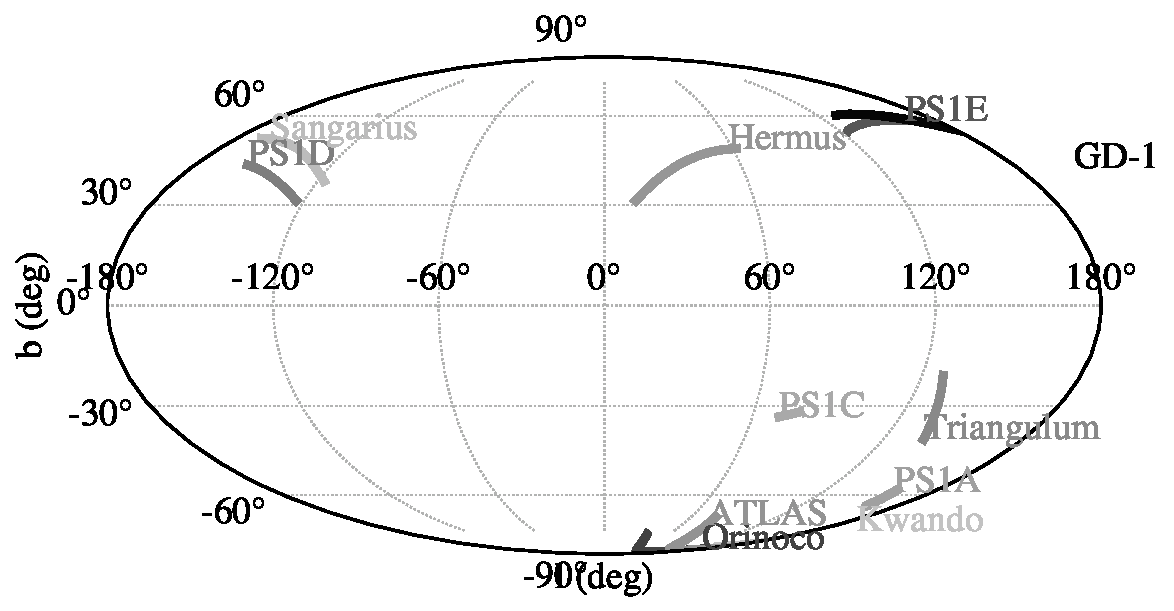
\includegraphics[width=0.7\textwidth]{sky_legend_gal1.pdf}
\caption{Comparison of precision in different model parameters attainable by 6-D observations of different streams.
Each panel shows on-sky positions of the analyzed streams, color-coded by the relative precision of a model parameter indicated in the upper right corner, with parameters on the bulge and the disk on the left and the halo parameters on the right.
Most of the baryonic parameters are set by the prior ($10\%$), which is only improved upon for the disk mass (middle left).
The constraints on halo parameters were obtained without including prior information, and are more diverse, even for streams that appear close in the sky.
Different streams are sensitive to different parameters, although no stream in this sample manages to constrain the scale radius better than $20\%$.
}
\label{fig:sky_precision}
\end{center}
\end{figure}

Figure~\ref{fig:sky_precision} summarizes \CRLB\ from fiducial 6D observations on all model parameters that streams in our sample have in common.
Each panel in a grid shows positions of streams on the sky (in galactic $(l,b)$ coordinates), colored by the fractional CRLB on the parameter indicated in the upper right corner of the panel.
The larger panel in the bottom has the scale and labels for each stream.
Similar to Figure~\ref{fig:crb2d_comparison}, the color-bar saturates at 20\,\% to highlight parameters for which streams provide interesting constraints.
Across the different parameters, streams provide diverse constraints: some parameters are constrained to the same degree by all of the streams, while there is variance from a few percent to more than 20\,\% for others.

In addition to stream observations, the bounds on baryonic parameters were informed by a 10\,\% prior, so the \CRLB\ on these parameters are better than 10\,\% for all of the streams.
To identify parameters whose bounds are determined predominantly by prior information, we calculated Kullback--Leibler divergence (KLD) between the prior and the bound:
\begin{equation*}
D_{KL} = \int_{-\infty}^{\infty} p(x) \ln\frac{p(x)}{q(x)} dx
\end{equation*}
where $p(x) = \mathcal{N}(0,\sigma_{bound})$ is the normal distribution centered on zero, with the parameter's \CRLB\ as a dispersion, and similarly $q(x) = \mathcal{N}(0,\sigma_{prior})$ is the normal distribution used as a prior on that parameter in the calculation of the \CRLB.
In general, KLD compares how similar two distributions are, so in our case, a small divergence means that the bound contains little information from streams.
Quantitatively, we call a parameter constraint prior-driven if its KLD with respect to the prior is smaller than $D_{KL}<0.01$, and plot these bounds with dotted lines in Figure~\ref{fig:sky_precision}.
None of the streams improved upon the prior information for the length scale of the bulge and disk, only several have improved on the bulge mass measurement (the inner halo streams GD-1, Hermus, Orinoco, and PS1A), while all the streams have constrained the disk mass further.
Mock streams in our sample are sensitive to the overall mass in the baryonic components, but not to its spatial distribution, which is likely a result of them never reaching closer than 4\,kpc from the Galactic center.
In the rest of the study, we focus on parameters for which streams provide constraints: the mass of the disk, and the halo parameters.


- another global observation: none of the streams constrains halo scale radius better than 20\%
- mixture for Vh, qx, qz, but no obvious trends with position on the sky
- on the contrary, some streams that appear in similar regions of the sky have very different sensitivity to halo parameters (e.g., qx for nearly parallel sangarius and ps1d separated by 5\,deg are x and y\%, respectively)
- so we next discuss how these depend on orbital properties

\begin{figure}
\begin{center}
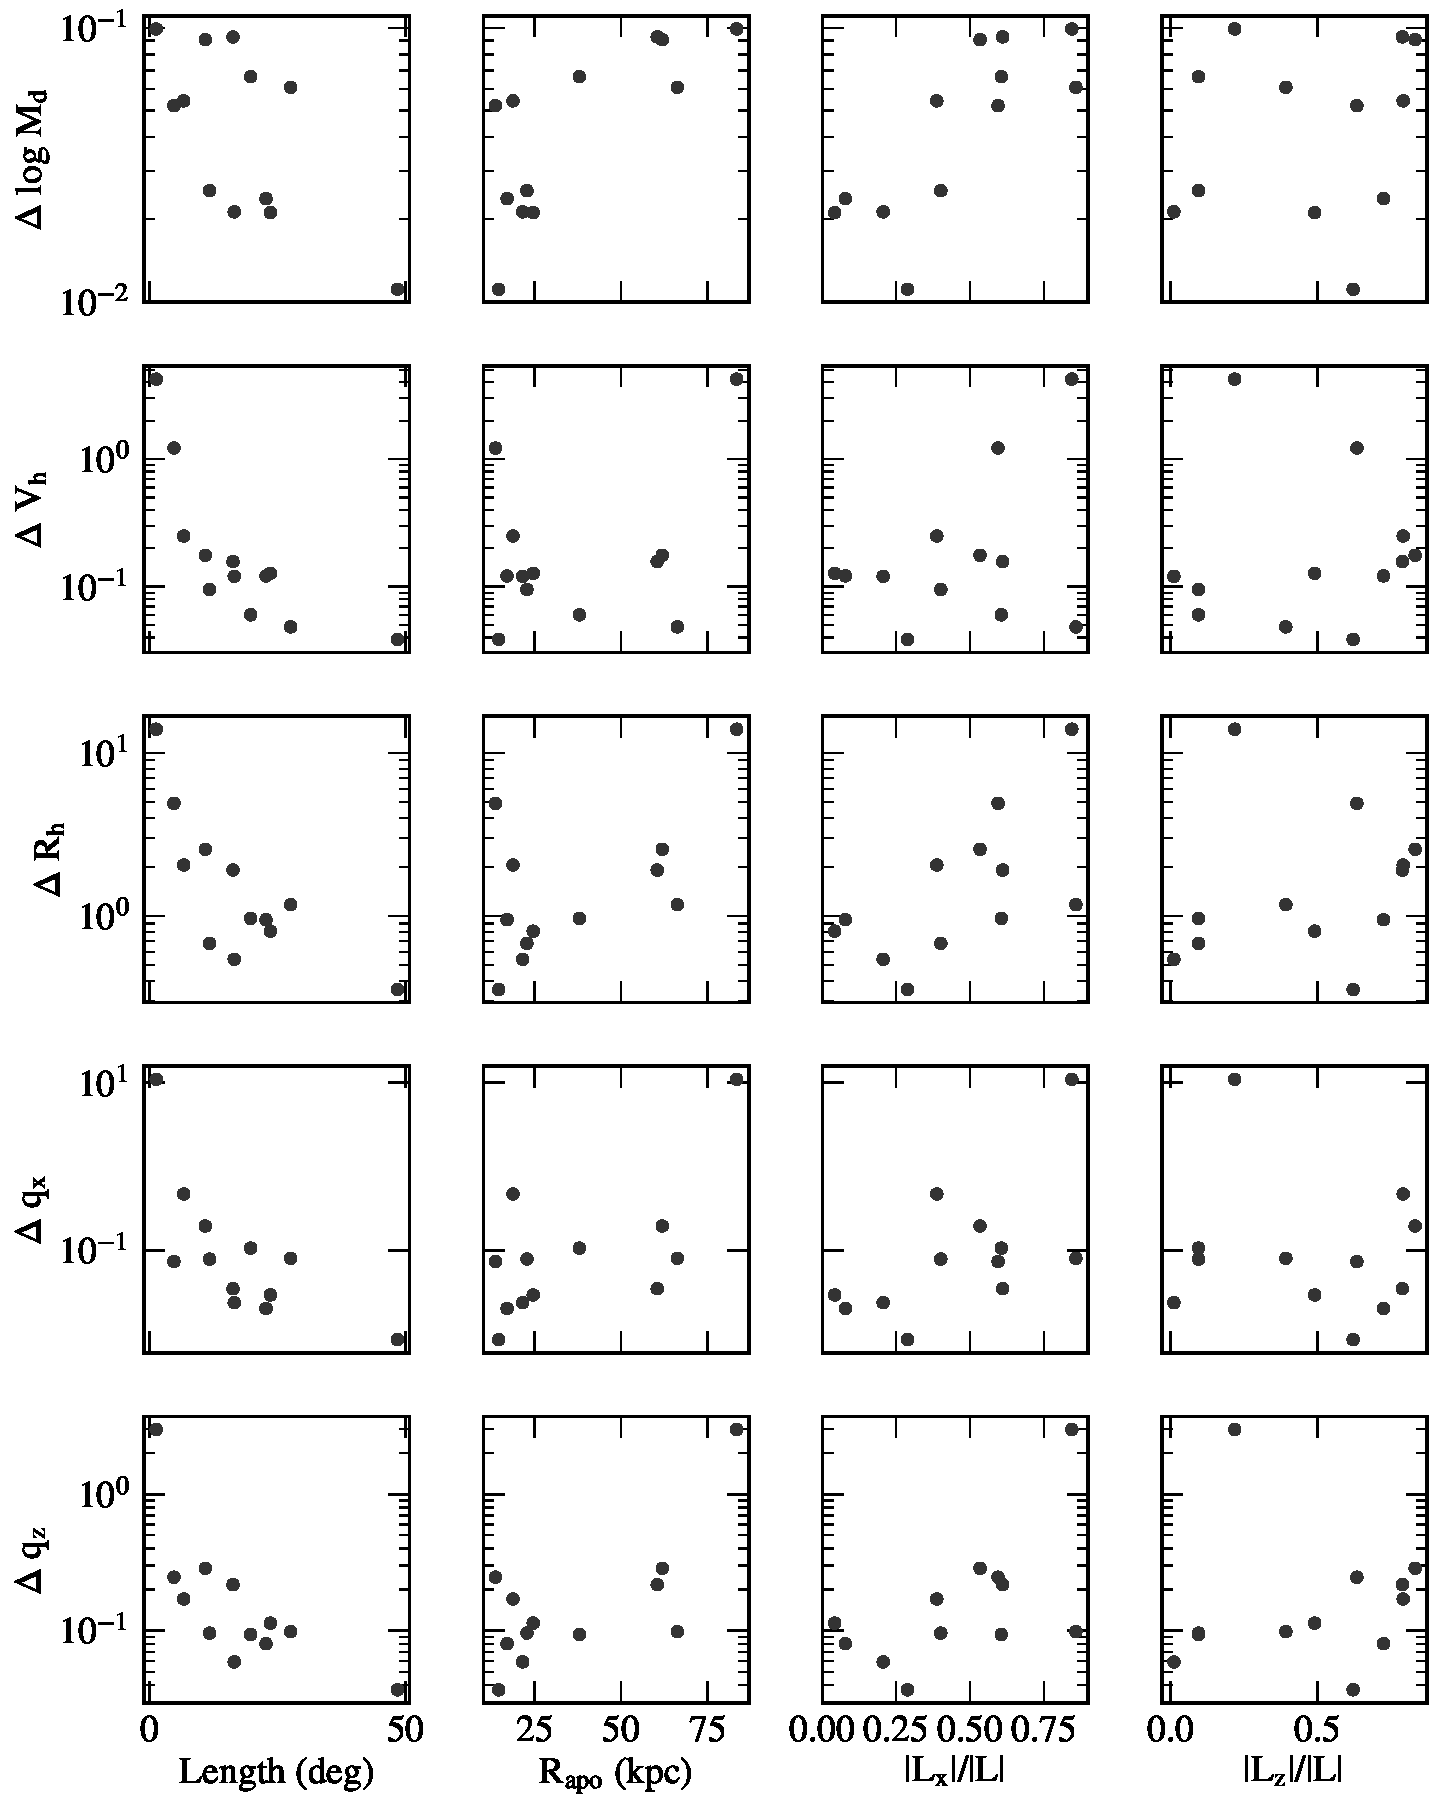
\includegraphics[width=\textwidth]{orbit_correlations.pdf}
\caption{Dependence of the precision in recovery of different model parameters (rows, from top: disk mass, halo scale velocity, halo scale radius, halo $x$ and $z$-axis flattening) as a function of different stream properties (columns, from left: stream length, apocentric radius, median $x$ and $z$-components of the angular momentum).
The most robust trend is with stream length, as long streams in general produce more precise constraints.
The disk mass is better constrained by streams whose angular momentum vector is in the disk plane.}
\label{fig:orbit_correlations}
\end{center}
\end{figure}



\subsection{Joint constraints}
\label{sec:res_joint}
% - CRB on halo parameters using different combinations of streams

\begin{figure}
\begin{center}
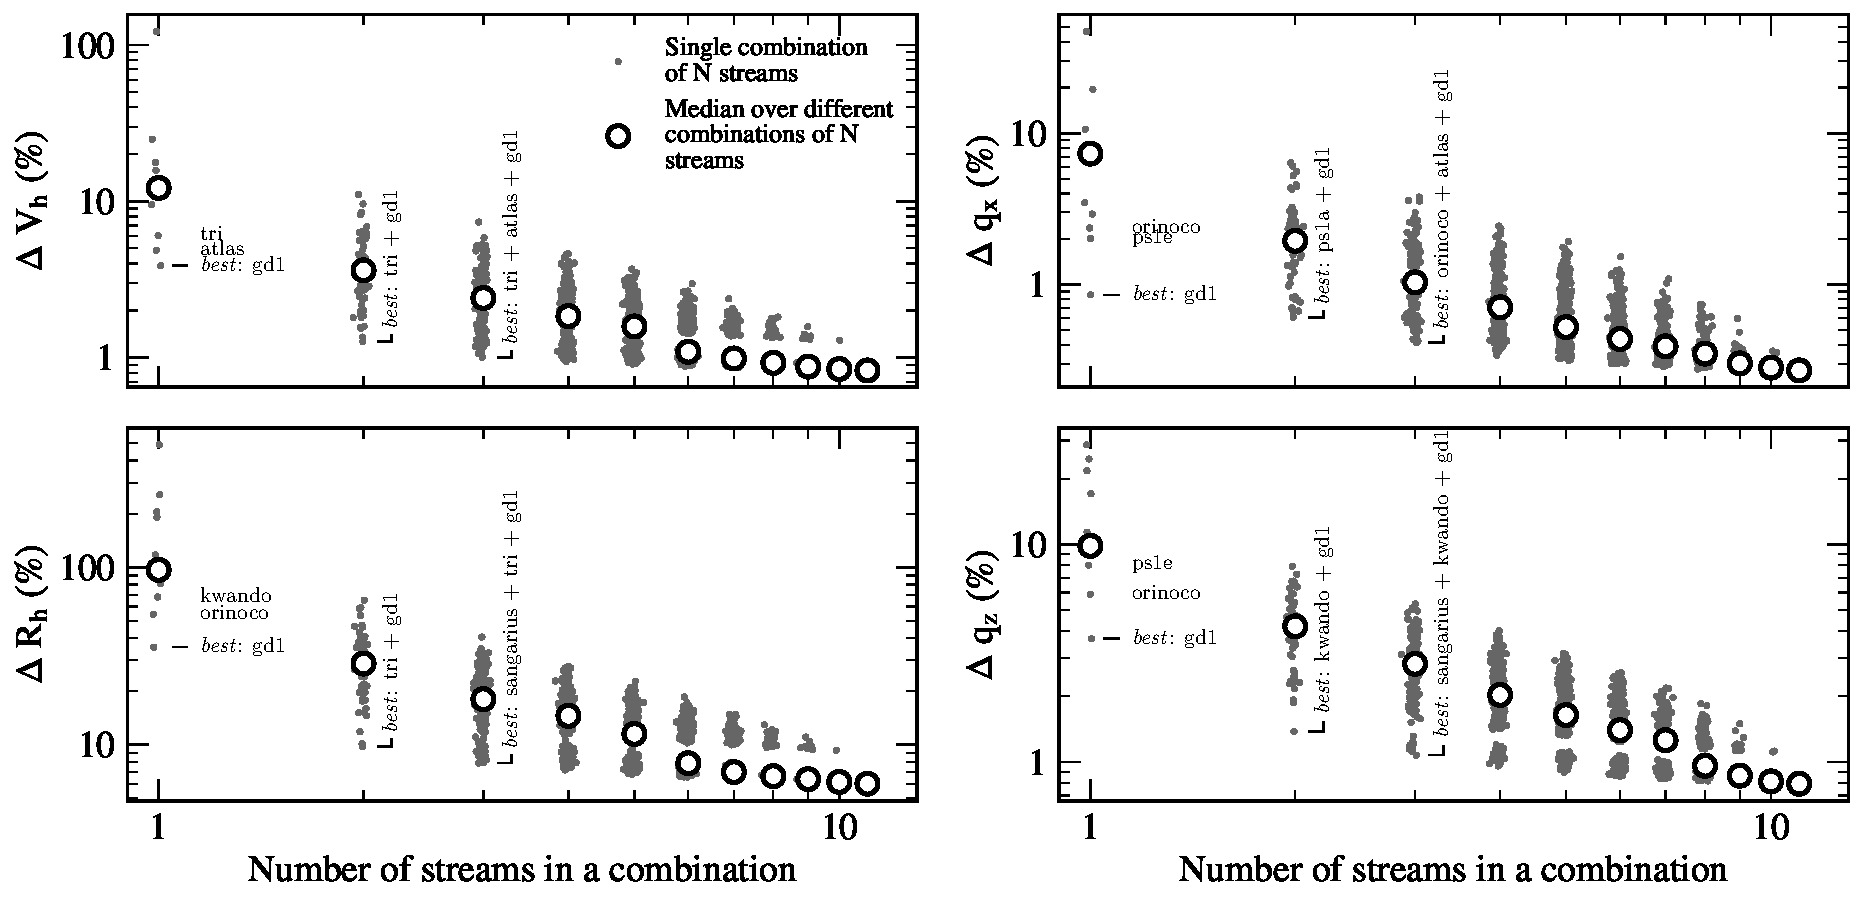
\includegraphics[width=\textwidth]{nstream_improvement.pdf}
\caption{Constraints on halo parameters improve when multiple streams are combined.
Each panel shows Cram\'er--Rao bounds on a halo parameter, as a function of the number of streams used to derive the bounds.
Gray points show constraints from a single combination of streams, while white points are the median across all the possible combinations for a given number of streams.
Combining any ten streams would provide percent-level precision in all parameters, except the scale radius, which is constrained at the $\sim10\%$-level.
We also label the three streams with best individual constraints on halo parameters, the best pair and the best triple.
For the scale velocity, the best pair and triple are a combination of the streams that have best individual constraints.
However, for the halo shape parameters, combinations of the best individual streams do not provide the tightest pair or triple constraints, indicating that streams compound the information content in non-trivial ways.
}
\label{fig:nstream_summary}
\end{center}
\end{figure}

\section{Applications}

\subsection{Forecasting and observation planning}
\label{sec:forecast}
\begin{figure}
\begin{center}
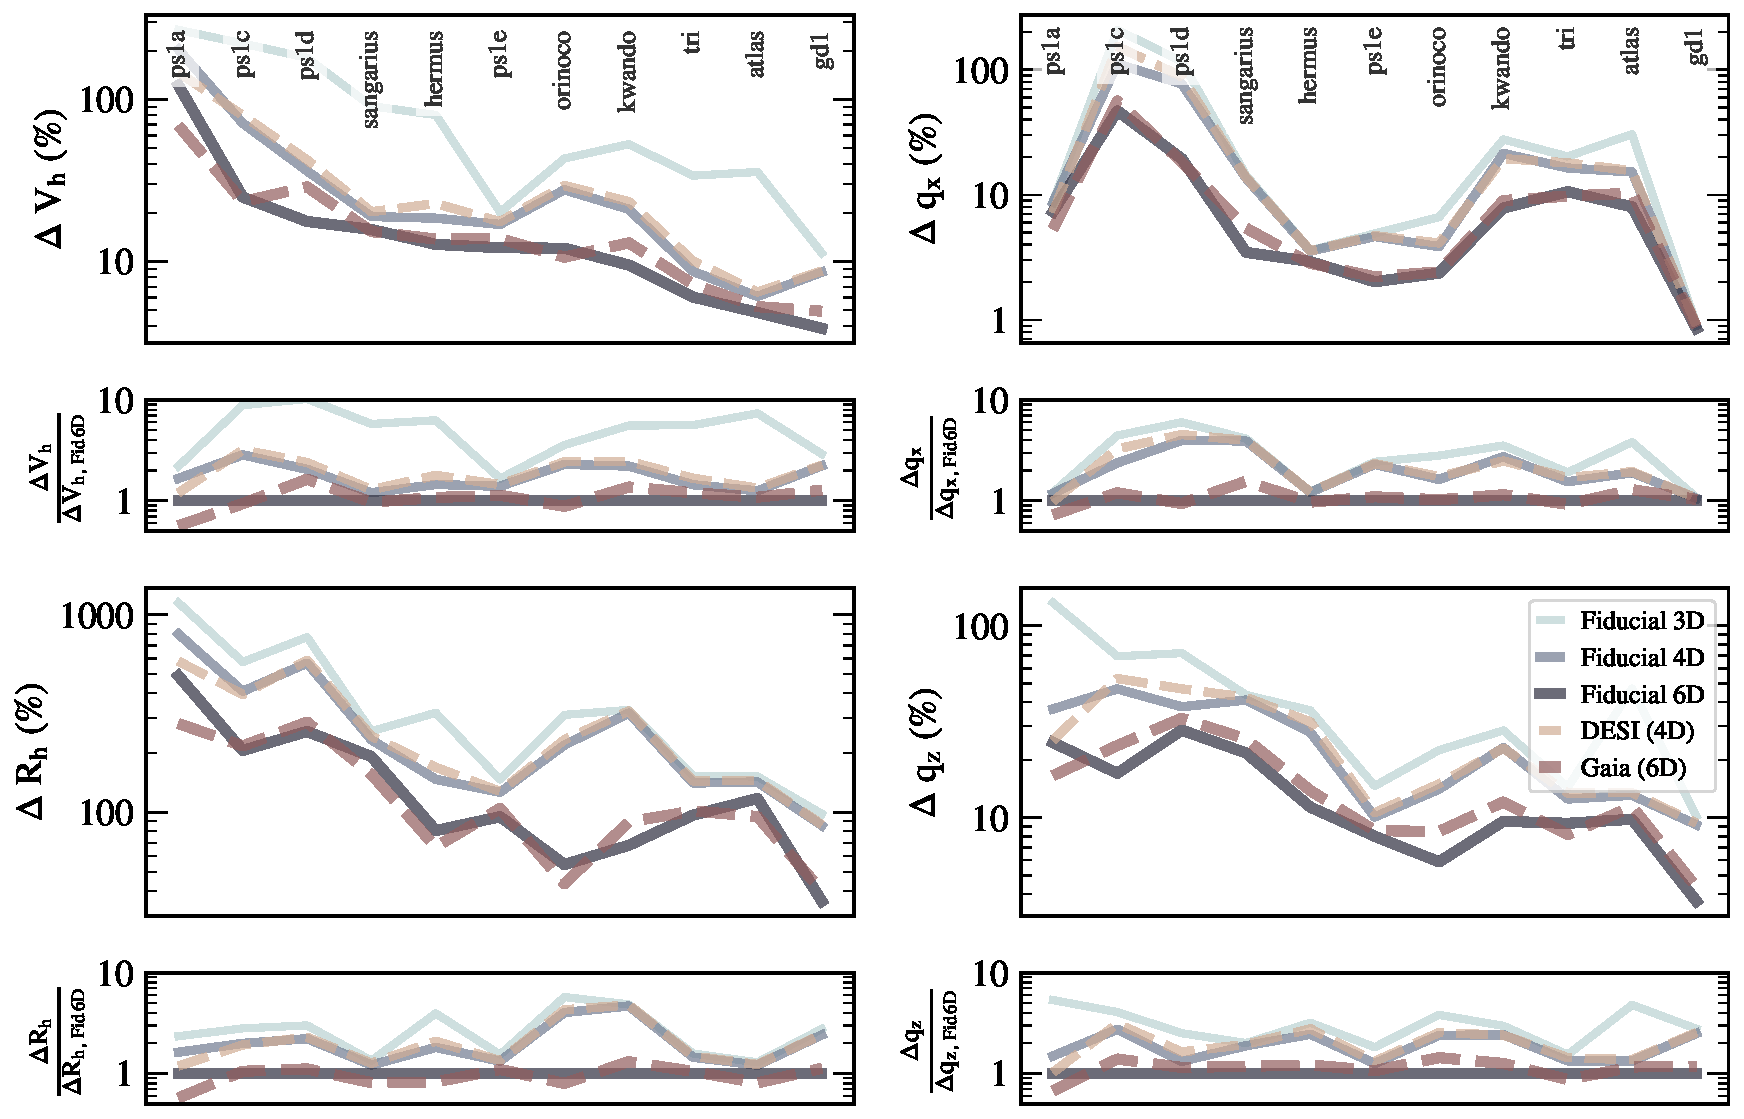
\includegraphics[width=0.7\textwidth]{../plots/obsmode_comparison.pdf}
\caption{Cram\'er--Rao bounds are valuable for planning observations, and in this figure we explore how the precision in recovered potential parameters (y axis) changes for different observing setups (different lines), for all the streams in our sample.
Each panel shows constraints on a single halo parameter (from top to bottom: halo scale velocity, scale radius, x-axis and z-axis flattening) from different streams, placed along the x-axis, and labeled in the bottom panel.
In general, constraints get better when the 3D positions are complemented with radial velocities (4D) and proper motions (6D), however, the magnitude of the improvement varies among the streams, as does the relative importance of having 4D versus 6D data.
We also note that observing modes with the same dimension of data, but different observational uncertainties (lines of different colors, but same width), produce similar constraints on halo parameters, hinting that the measurement uncertainty is of secondary importance. 
}
\label{fig:obsmodes}
\end{center}
\end{figure}

% - different observing modes
% - raise issue of member identification, which was not addressed here

\subsection{Physical interpretation of constraints}
\label{sec:interpretation}
- potential == theoretical construct, matter field physical
- density / enclosed mass can be calculated given parameters of the potential by integrating the poisson's equation
- the bounds are then propagated using eqn:

- however, density / enclosed mass is an integrated property, no/hard? to analytically calculate
- on the other hand, radial acceleration is straightforward -- just differentiating the potential
- it also correlates with enclosed mass (and in spherically symmetric case ?), so use ar as our proxy of a physical quantity

\begin{figure}
\begin{center}
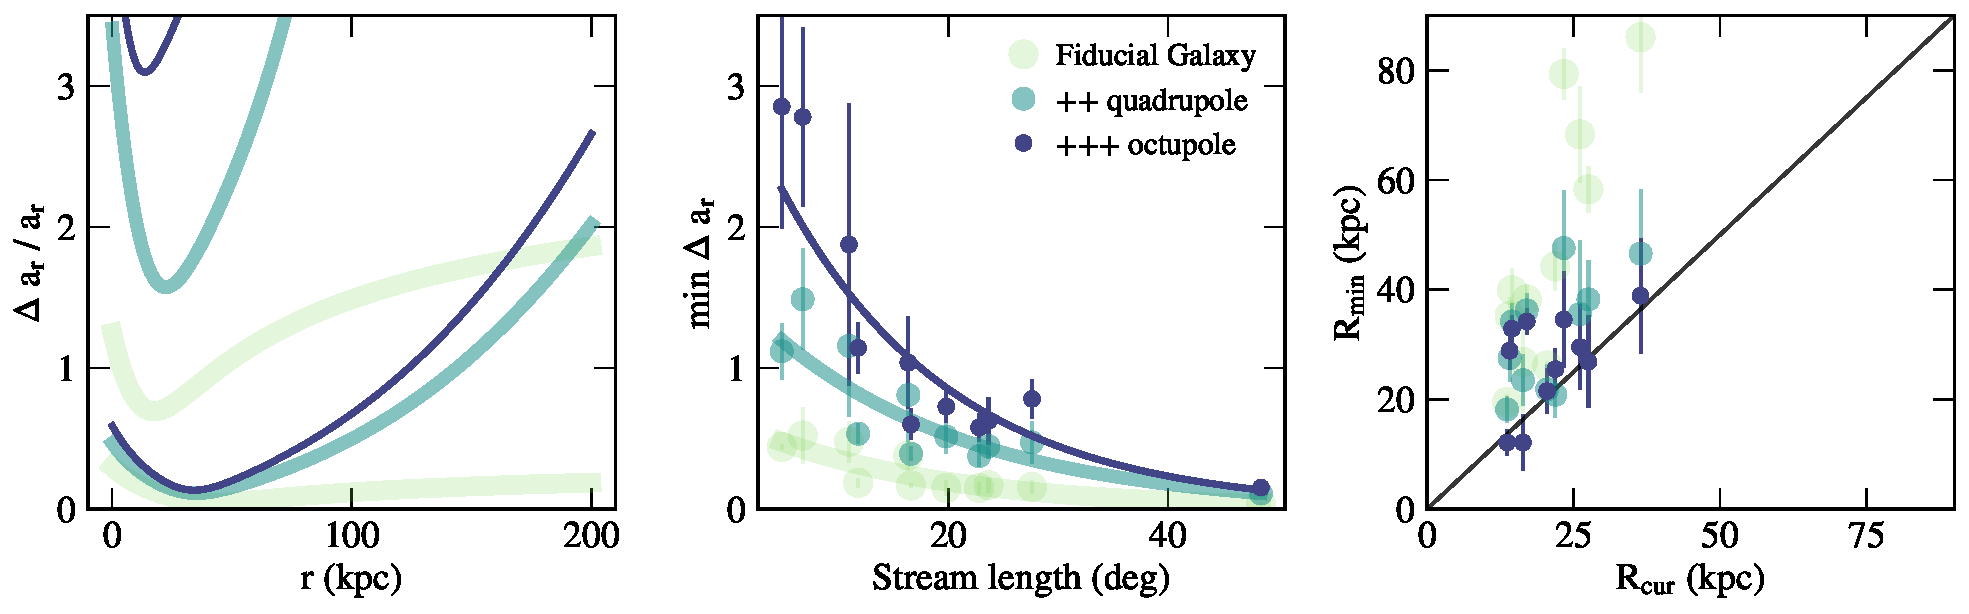
\includegraphics[width=\textwidth]{ar_crb_all.pdf}
\caption{Fractional constraints on the circular velocity by 6-D phase space data on stellar streams (with lighter colors representing streams with larger apocenters).
Precision in recovered circular velocity as a function of distance from the Galactic center (\emph{left}).
Streams vary in their ability to constrain circular velocity (thicker lines are used for more competitive constraints), but all have a single Galactocentric distance where the constraint is maximized.
Long streams provide tighter constraints (\emph{center}), while the location of the best constraint correlates with the orbital apocenter (\emph{right}).
}
\label{fig:ar}
\end{center}
\end{figure}

- top row of Figure~\ref{fig:ar} shows in fiducial case fractional constraints on radial acceleration as a function of distance from the center along a random line of sight
- different lines for different streams -- different scales and normalizations, but all show a local minimum
- in the second panel we show that the best constraint is a strong function of the stream length, consistent with findings for original parameters of the potential field
- errorbars are 16th to 84th percentile across the 50 different sightlines
- in the two right-most panels we explore where the best measurement of the acceleration is obtained, by plotting the minimum of Delta ar curves as a function of current radial distance of the stream (second panel from the right) and apocentric radius (first panel on the right).
- the positions of best stream constraints are scattered off the one-to-one line (solid black), but in general seem to correlate with apocenter
- the correlation with current position is very non-linear

- however, the fiducial model is parametric -- rigid, meaning that getting one thing right gets many other things right as well
- if the best measurement is truly attained at the apocenter, that would mean that the streams at the present contain the information on their whole orbital history, constraining the total enclosed mass within their apocentra.
- alternatively, if the best measurement is at the current position, that means that streams are foremost a local measure of the enclosed mass.
- these are radically different interpretations, so in the final application of our framework to measure information content in streams, we relax our assumptions about the potential and show what properties of more flexible potentials are constrained by stellar streams

\subsection{More flexible potential models}
\label{sec:bfe}
- in this section, we expand on the basic model of the Galaxy studied throughout this work
- in particular, we consider the influence of an external multipole, whose contribution to the potential field is given by eqn:
- where $a_{lm}=0$ are coefficients of the spherical Bessel functions
- we are expanding around our fiducial model, so $a_{lm}=0$, however, we leave them as free parameters, and measure how well the streams constrain them
- we go up to the octupole moment, $l=3$, which adds up 15 additional parameters to our model

- bottom row of Figure~\ref{fig:ar} shows constraints on radial acceleration in the case where the potential gets progressively more complicated: fiducial in light green, with added dipole in dark green, up to quadrupole in blue and up to octupole in purple
- as expected when adding more parameters to the model, overall the model is less constrained
- for simplicity, we only show delta ar(r) for a couple of streams, and see that \CRLB\ increase in more flexible potentials
- this is also confirmed for all of the streams in the second panel from the left, where we show how the constraints depend on the stream length
- while all streams produce weaker constraints in more flexible models of the Galaxy, the performance decreases exponentially? for short streams
- however, the constraints also become more localized, because the delta ar(r) curves on the first panel have a deeper minimum -- which means that the streams only know about region of the Galaxy 
- and that turns out to be the local position; third panel shows that in the octupole case, best ar constraints for all but a few streams are within $1\,\sigma$ of the current position

- powerful finding: streams constrain the mass enclosed within their current position, with a precision determined by their length
- both of these are observables, so we can easily predict what kind of object would give what kind of constraint
- while we clearly see trends with orbital properties, such as eccentricity, they are less important 

% - end with the need for a model that is both flexible spatially and realistic (ie, has a good basis, but also evolves in time)
% - can we make the case with ophiuchus, or perhaps some of the streams close to the LMC?
% - posit whether galaxy simulations would provide good models, or just a basis in which we evolve individual subhalos


\section{Discussion}
\label{sec:discussion}
% - context of stream constraints so far
% - improvement in gd1+pal5 as expected?
% - similarly, pal5+ngc5466 from lux prediction as ours?


\section{Summary}
\label{sec:summary}


\emph{Acknowledgements:} This work was improved upon following the thoughtful suggestions of the Conroy group, the Finkbeiner group, Dan Foreman-Mackey, Kathryn Johnston, Nikhil Padmanabhan, Adrian Price-Whelan and Hans-Walter Rix, and it is a pleasure to thank them.

\bibliographystyle{aasjournal}
\bibliography{crlb}

\appendix
\section{Cold tidal streams in the Milky Way}
\label{sec:streams}

Steps for creating a mock stream:
\begin{itemize}
 \item obtain ridge points along the stream. This is done either by analyzing a match-filtered map showing the stream, or from published stream tracks (usually in a polynomial form).
 \item fit a polynomial to the ridge points, and define a stream coordinate system with one axis along the polynomial, and the other along the normal on the polynomial.
 \item query PanSTARRS1 star catalog and assign a membership probability. We assume that the total probability can be split in a spatial and color-magnitude component; $p = p_{spatial} \times p_{CMD}$. The spatial probability follows a normal distribution centered on the stream track (measured as described above), with dispersion matching the reported stream width. The color-magnitude probability is obtained from a matched filter based on the M13 globular cluster, and placed at the reported distance to the stream.
 \item select a hundred most likely members. If kinematic information is present, the lowest probability members are replaced by stars with kinematic measurements.
 \item these hundred members are then used to constrain parameters of the mock stream progenitor. The mock stream is created in a fiducial gravitational potential defined by the first 9 parameters listed in Table~\ref{t:model} and these parameters are kept fixed for all of the mock streams. The variable parameters are: 6D position of the progenitor today, initial mass of the progenitor (we assume the progenitor loses mass at a constant rate and disappears at the present, with the exception of Pal~5 and NGC~5466, where we use the present-day cluster mass), and the age of the stream. 
\end{itemize}


\begin{figure}
\begin{center}
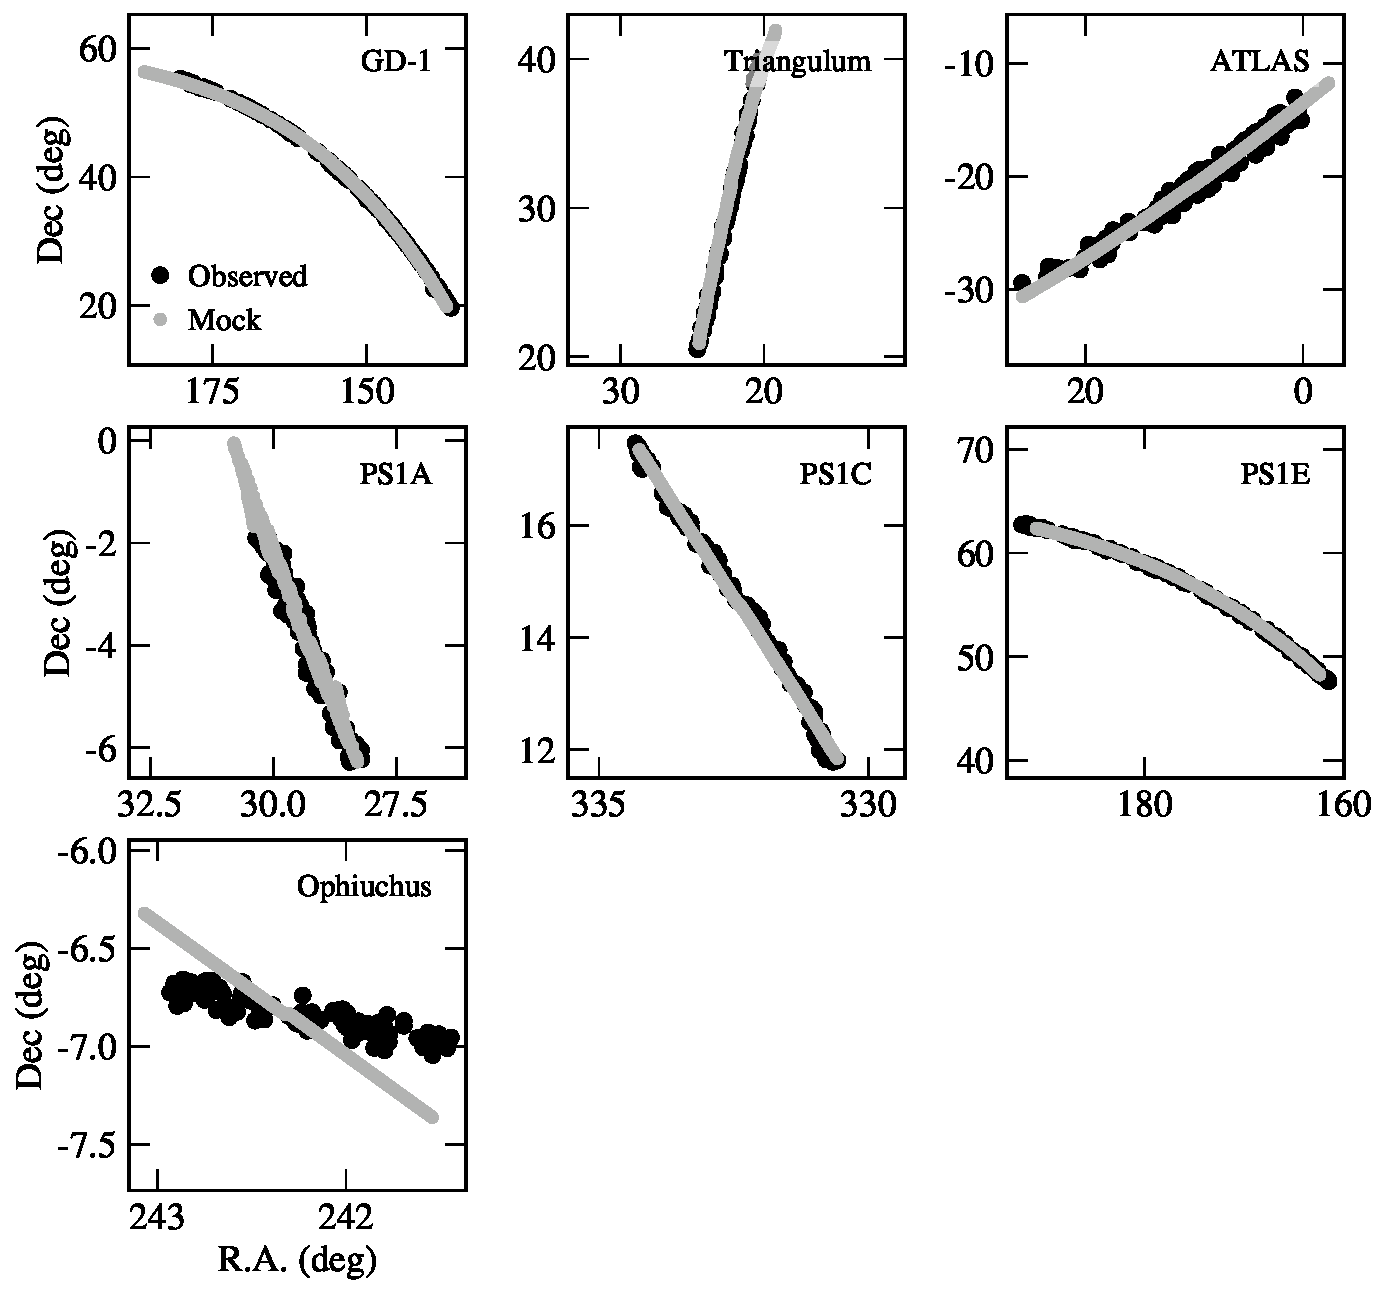
\includegraphics[width=\textwidth]{mocks.pdf}
\caption{On-sky positions of streams analyzed in this work, with one stream per panel, and the stream name in the upper right corner.
In each panel, the observed stream members are shown in black, whereas a best-fitting mock stream is plotted in gray.
All of the mock streams have been generated in the same gravitational potential, and they fit the observations reasonably well.
Streams where the mock deviates from observations likely experienced a different gravitational potential for at least a part of its evolution.
}
\label{fig:gallery}
\end{center}
\end{figure}

\section{Robust matrix inversion}
\label{sec:inversion}
Inverting a Fisher matrix is a core operation in calculating Cram\' er--Rao lower bounds and thus measuring the information content in stellar streams. 
Often, this problem is ill-conditioned, i.e. if the input Fisher matrix $I$ is modified only slightly, the standard numerical algorithms, such as that employed in \texttt{numpy.linalg.inv}, return a very different inverse $I^{-1}$.
We adopt an iterative approach of rescaling the problem to ensure a robust inverse is obtained, and outline it below.

Starting with a matrix $A$, which may have a large condition number, we are looking for a matrix $Q$, such that $Q A = I$.
If we have a guess for $Q$, and the guess is good, then the matrix $QA$ has a low condition number, and can be reliably inverted using the standard algorithm for numerical inversion.
Then it follows:
\begin{equation*}
(QA)^{-1} Q = A^{-1} Q^{-1} Q = A^{-1}
\end{equation*}
We have just obtained a better guess for the inverse of the original matrix $A$, and adopt it as the matrix $Q$ in the next iteration.
This procedure is repeated until $Q$ converges to $A^{-1}$, i.e., $Q A = I$ to machine precision.

In our current implementation, we use the standard, unreliable inverse as the starting guess $Q$. 
Convergence to the true inverse is typically obtained after several ($\lesssim2$) iterations.

\end{document}

